%% ===========================================================================
%%  Shared, class-independent body.  Both main.tex (neutral, local build) and
%%  main_sn.tex (Springer Nature sn-jnl, Overleaf) \input this file unchanged.
%%  Prose under sections/ is generated by build_tex.py from ../sections_en;
%%  sections/04_2_terrain_blending.tex is hand-authored (it carries the maths).
%% ===========================================================================

\section{Introduction}\label{sec:intro}
Autonomous lunar landing is a control problem with direct operational consequences: during the powered-descent phase it requires precise positioning and safe contact, in real time, over cratered, rocky, and sloped terrain. In recent years GPU-parallel physics engines (NVIDIA PhysX) and the simulation frameworks built on them have made it practical to learn complex, contact-rich tasks with deep reinforcement learning (RL) by running thousands of environments concurrently \citep{mittal2023,nvidia2025,rudin2022}. The project underlying this study belongs to that class: it is an Isaac Lab direct-workflow task in which a four-legged rocket with a two-axis gimbal-thrust engine learns, using the Soft Actor-Critic (SAC) algorithm, to land on a procedural lunar surface built from a real digital elevation model (DEM) macro surface enriched with craters, rocks, and centimetre-scale regolith texture.

In procedural multi-resolution terrain of this kind, two layers are typically used to keep the compute and memory budget bounded: a low-resolution global surface covering a wide area, and a high-resolution local patch generated only in the region near the agent or the target where it is needed. Seamlessly joining these two layers is a classic problem, studied in the computer-graphics literature for more than twenty-five years (geometry clipmaps: \citealp{losasso2004}; ROAM: \citealp{duchaineau1997}; geomipmapping: \citealp{deboer2000}). That literature, however, focuses almost entirely on rendering quality; how a discontinuity at the join boundary affects foot-to-ground contact, altimeter readings, or the noise character of an RL agent's proprioceptive observation is rarely addressed quantitatively.

In the system studied here this problem appears with two distinct and mutually inconsistent solutions: the training environment blends between layers with a compact-support cubic \texttt{smoothstep} function, whereas a previously used mesh-based implementation uses an infinite-support Gaussian bell. These two functions differ in a fundamental mathematical property: \texttt{smoothstep} reaches exactly zero at a finite radius (compact support), whereas the standard Gaussian bell never reaches exactly zero at any finite radius (infinite support; \citealp{hardy1971}) and must be truncated somewhere to be usable in an engineering application; that truncation risks creating a new, measurable seam at the cut point. Comparing the two methods fairly requires forcing both to zero at the same transition radius (hard truncation) and measuring them under the same transition budget; this form of comparison is not directly addressed in any of the terrain-randomization studies surveyed here (see Section~\ref{sec:related}).

Motivated by these observations, this study addresses three research questions:

\begin{itemize}
  \item RQ1: When compared fairly under the same transition-radius budget, how large is the quantitative difference in boundary continuity (C0/C1) between compact-support (\texttt{smoothstep}) and infinite-support (Gaussian) blending functions, and what trade-off does this difference create with computational and memory cost?
  \item RQ2: Can a \texttt{hybrid} blending method that uses a Gaussian in the landing-gear contact region and \texttt{smoothstep} beyond it combine the continuity advantages of both methods at a reasonable increase in computational cost?
  \item RQ3: Do the continuity differences among these three blending methods translate into a measurable difference in learning performance in a real Isaac Sim/Isaac Lab SAC training run?
\end{itemize}

Accordingly, the aim of the study is threefold: (i) to compare the existing \texttt{smoothstep} method and the previously used Gaussian method quantitatively within the same architecture and under the same transition budget; (ii) to propose and validate a \texttt{hybrid} method that combines the advantages of both; and (iii) to compare these three methods not only at the analytic/CPU level but inside a real Isaac Sim/Isaac Lab GPU-parallel physics simulation, with a real SAC training run, and thereby show whether the choice of blending function is reflected in learning performance. This last point is central to the novelty of the study: the comparison is carried out not as an abstract numerical experiment but on real lunar terrain, inside a real Isaac Sim training loop.

The main contributions of this study are as follows:

\begin{itemize}
  \item The existing \texttt{smoothstep} and the previously used Gaussian blending methods are, for the first time, compared fairly under the same transition budget by truncating them at a finite transition radius (hard truncation); it is shown that the untruncated Gaussian appears well-behaved but in fact carries a hidden seam defect that emerges once it is truncated at a finite radius.
  \item A new \texttt{hybrid} blending method is proposed that uses a switch weighted toward a Gaussian in the contact region and toward \texttt{smoothstep} beyond it; this method is shown to provide continuity at machine precision and to create no new seam at its own internal transition.
  \item A statistically validated (Wilcoxon signed-rank test) comparison of continuity, cost, and VRAM is performed over thirty seeds and four method variants (\texttt{smoothstep}, as-shipped Gaussian, calibrated Gaussian, \texttt{hybrid}); the robustness of the findings is tested with four separate ablation analyses (contact radius, switch width, transition radius, grid resolution).
  \item The three methods are compared inside a real Isaac Lab/Isaac Sim PhysX environment, with GPU-parallel SAC training; unlike prior work in the terrain-randomization literature, this is the first attempt to treat the choice of blending function directly as a training-design variable.
  \item This real training comparison is run not with a single seed per method but with three independent seeds (n=3); by showing that the large apparent performance gap seen in the initial single-seed measurement cannot be confirmed statistically with multiple seeds, the study provides a concrete, self-sourced cautionary example about the reliability of single-run RL comparisons.
  \item All three methods are integrated into the production code in a backward-compatible way (without changing existing behaviour) and are selectable via an environment variable (\texttt{ISAACLAB\_TERRAIN\_BLEND\_METHOD}).
\end{itemize}

The remainder of this paper is organized as follows. Section~\ref{sec:related} reviews the literature in which the study is situated, under five thematic clusters. Section~\ref{sec:method} details the experimental environment and the simulation setup shared by all runs, the mathematical definition of the blending functions, the analytic evaluation protocol, the reinforcement learning method used (the task's MDP formulation and SAC), and the real Isaac Sim training protocol. Section~\ref{sec:results} presents the continuity, cost, VRAM, ablation, and real training results. Section~\ref{sec:discussion} discusses the findings in relation to the literature and addresses the limitations. Section~\ref{sec:conclusion} summarizes the study and closes with concrete directions for future work.


\section{Related Work}\label{sec:related}
This section reviews the literature in which the study is situated, under five thematic clusters. The review is a targeted (scoping) review; it is not a PRISMA-compliant systematic review, and within each cluster the most-cited/foundational references of the field are prioritized.

Cluster 1 concerns multi-resolution blending and level-of-detail (LOD) transitions in procedural terrain. Geometry clipmaps \citep{losasso2004}, ROAM \citep{duchaineau1997}, and geomipmapping \citep{deboer2000} form exactly the traditional computer-graphics lineage to which this study's two-mesh (global + local patch) framing belongs; all three treat the formation of cracks/seams at the boundary where a low- and a high-resolution mesh meet as a central engineering problem; \citet{pajarola2007} survey this family of semi-regular multiresolution models in full. The problem has not been retired by newer pipelines: \citet{zhang2019} report that transitions between levels are still usually not handled well, producing popping artefacts, and address them with dynamic stitching strips, while \citet{jain2024} attach a learning-based level-of-detailing stage to a quad-tree terrain renderer. What all of this work optimizes, however, is what the transition looks like, not what a physics query returns at it. This study's finding~--- that the as-shipped Gaussian leaves a real seam when truncated at a finite radius~--- is a concrete, measured instance of the same class of problem this literature has been trying to solve for more than twenty-five years; and \texttt{smoothstep}'s compact support coincides with the principle, used by ROAM and geoclipmaps, of a weighting function that goes exactly to zero at the boundary.

Cluster 2 concerns the continuity properties of compact-support and infinite-support blending functions. The multiquadric/Gaussian-type radial basis function that \citet{hardy1971} proposed for topography is, like the family to which this study's as-shipped Gaussian belongs, infinite-support and never reaches exactly zero at any finite radius; this is consistent with the measured residual behaviour (approximately exp(-1) \textasciitilde{} 37\%). \citet{wendland1995} formalizes the solution: compact-support, minimal-degree positive-definite radial functions for a given smoothness order; \texttt{smoothstep} (cubic Hermite, \citealp{ebert2002}) is a one-dimensional, low-degree special case of this family. \citet{ohtake2003} describe the strategy followed by this study's \texttt{hybrid} method: building a multi-scale hierarchy from compact-support basis functions to obtain different blending behaviour at different scales.

Cluster 3 concerns terrain modelling and contact dynamics in planetary/lunar landing simulations. The goal of the ALHAT program \citep{johnson2008,nasajpl}~--- precise landing within one hundred metres and LiDAR-based terrain-relative navigation~--- and the accuracy level offered by LOLA/SELENE-based digital elevation models \citep{barker2016} show that in real lunar-landing engineering, terrain accuracy is not cosmetic but a direct operational requirement. This strengthens the study's "why seams/continuity matter" motivation: a discontinuity in the foot contact region corresponds, in real ALHAT-class systems, to a class of error that can affect hazard-detection and landing-site-selection decisions. This motivation is also corroborated by recent flight data: the vision-based navigation and obstacle-detection results of JAXA's SLIM mission (January 2024; \citealp{ishida2025}) showed that real-time obstacle/terrain detection performed 50 m before landing yielded metre-level landing precision~--- concretely demonstrating that errors in terrain representation are reflected directly in landing safety not only in simulation but in real flight. The contact side carries the same sensitivity: using discrete-element analysis, \citet{nakashima2010} show that the drawbar pull and sinkage of a small lunar rover wheel depend strongly on the local slope geometry it actually meets, which is precisely the quantity a seam perturbs. On the learning side, \citet{scorsoglio2021} train image-based deep reinforcement meta-learning policies for autonomous lunar landing, but on rendered imagery rather than on a contact-resolved physics surface, so the geometry of the join never enters their evaluation.

Cluster 4 concerns procedural terrain randomization in physics-based RL environments. \citet{rudin2022} use, on IsaacGym, a difficulty-based terrain curriculum similar to the terrain pool in this study; this shows that the study's curriculum and terrain-pool design is not an isolated instance but an established practice in the field. \citet{mittal2023} and \citet{nvidia2025} define the architectural basis of the very platform this study uses, while \citet{tobin2017} provide the general motivation for procedural randomization in sim-to-real transfer. \citet{muratore2022} survey robot learning from randomized simulations and catalogue the randomization axes used in practice, and \citet{collins2021} compare the physics simulators these pipelines are built on, noting how seldom contact-level fidelity choices are reported quantitatively. Closest to this study's platform, \citet{richard2024} present OmniLRS, an Isaac-Sim-based photorealistic lunar simulator assembled from a real DEM macro surface plus procedural fine detail~--- the same two-layer construction used here~--- but evaluate it for rover perception rather than for the contact geometry a lander's foot meets. None of these sources, however, treats the multi-resolution blending function itself (\texttt{smoothstep}, Gaussian, or \texttt{hybrid}) as a design variable within terrain randomization; all focus on terrain diversity, not on the effect of the blend shape on continuity and learning cost. This study is positioned precisely in that gap.

Cluster 5 concerns \texttt{hybrid}/regional combination of blending functions (partition of unity). \citet{ohtake2003} are again the central source here: the multi-scale, partition-of-unity-style combination of compact-support basis functions is the general mathematical framework of this study's \texttt{hybrid} method (one function in the contact region, another beyond it, with a smooth switch between them). The canonical statement of that framework is the multi-level partition of unity implicit \citep{ohtake2003mpu}, in which locally fitted functions are blended by smooth, compactly supported weights that sum to one at every point~--- exactly the role played here by the pair switch(r) and 1 - switch(r). Under this framework, the \texttt{hybrid} switch not creating a new seam at machine precision is an expected result consistent with the literature: the convex combination of two C1-smooth functions with a C1-smooth weight is again C1-smooth.

In summary, Cluster 1 supplies the problem class (seams/continuity in multi-resolution transitions) but this literature is largely focused on visual quality; this study measures the same problem numerically on a physically queryable height field (foot contact). Cluster 2 grounds why the empirical finding is correct in a mathematical result more than fifty years old; this is not a coding error but a known structural property of radial basis functions. Cluster 3 provides real-world engineering justification for the "why does it matter" question. Cluster 4 clarifies where this study's experimental platform sits in the literature and the gap it fills. Cluster 5 moves the proposed \texttt{hybrid} method from being an isolated engineering trick to sitting within an established mathematical framework.


\section{Method}\label{sec:method}
This section consists of six subsections: the experimental environment and task definition, the simulation setup shared by all runs, the terrain representation and the mathematical formulation of the blending problem, the analytic (CPU) evaluation protocol, the reinforcement learning method used (the task's formulation as a Markov decision process and the Soft Actor-Critic algorithm), and the real Isaac Lab/Isaac Sim training protocol. All three blending methods were evaluated first at the analytic/CPU level and then inside the real GPU-parallel physics simulation, under the same fixed transition radius and the same hard-truncation rule; this consistency makes the findings comparable across the two evaluation layers. Figure~\ref{fig:flow} summarizes this pipeline, from terrain generation through the choice of blending function to the analytic evaluation and the real training analysis.


\begin{figure}[htb]
  \centering
  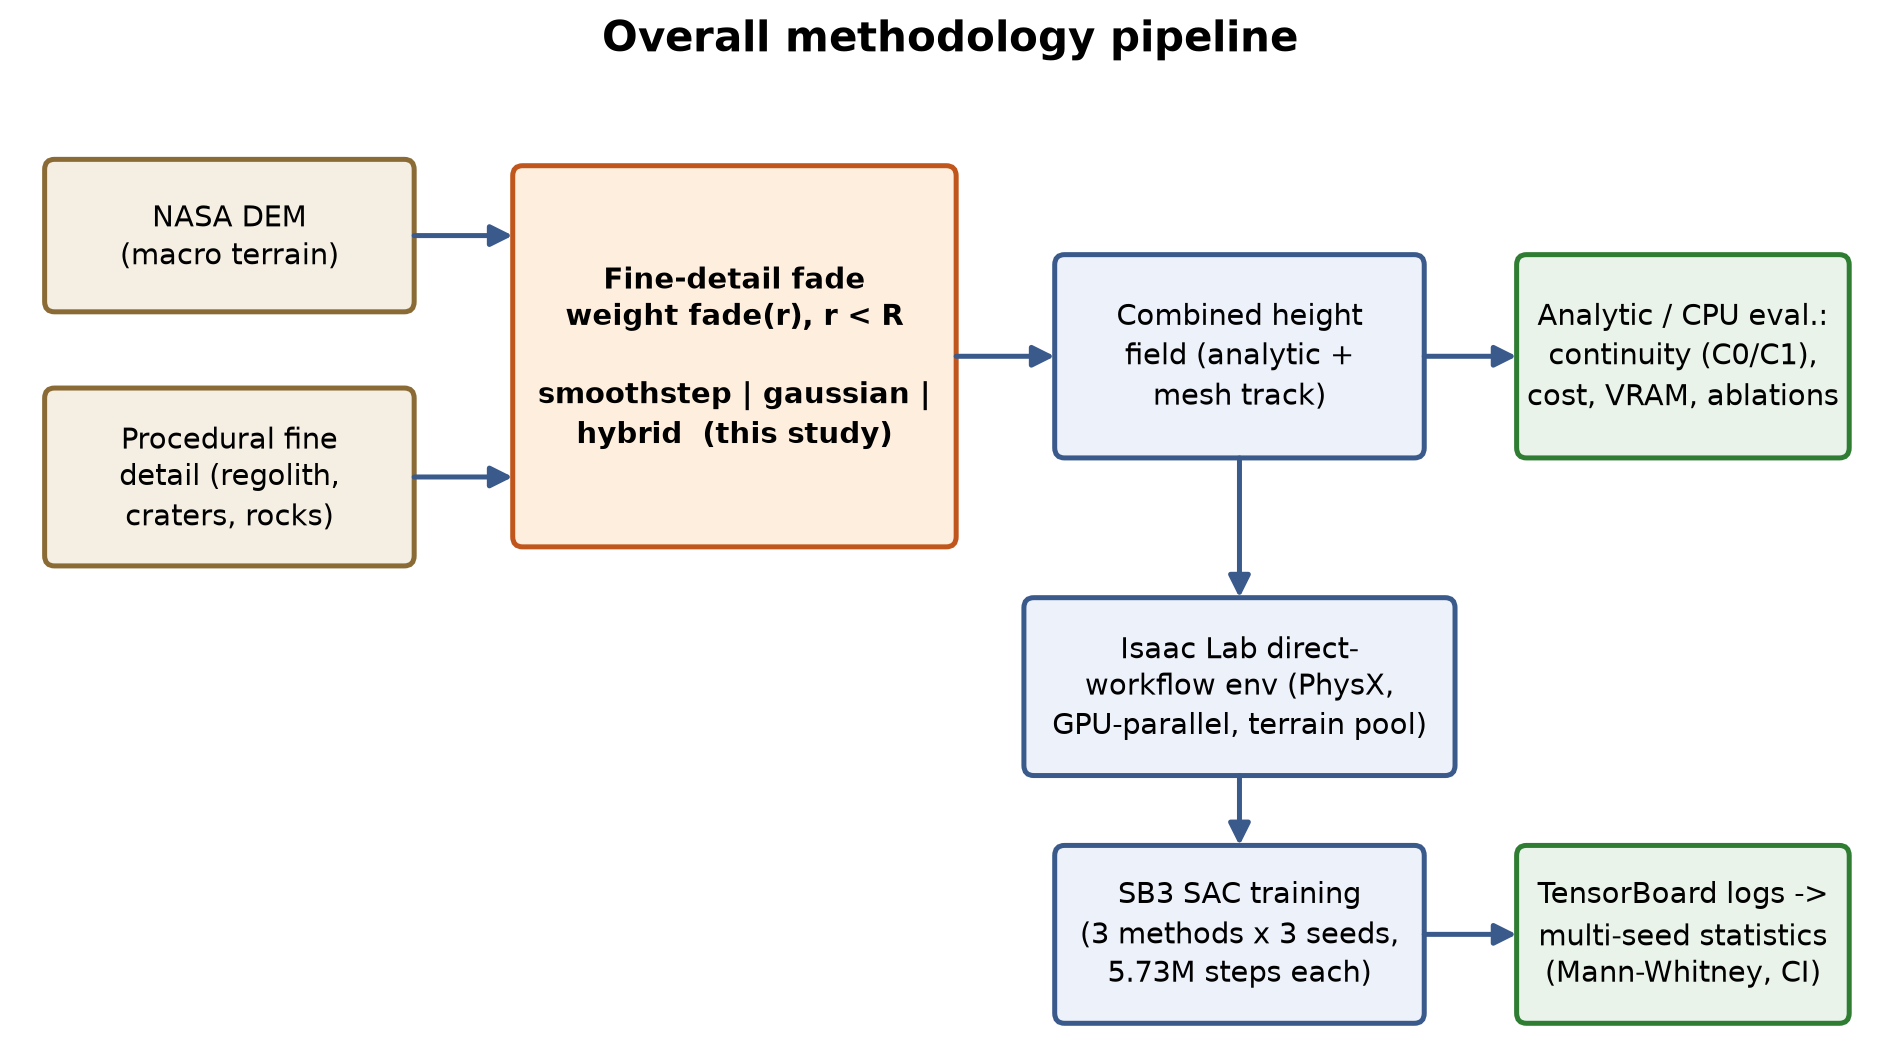
\includegraphics[width=\linewidth]{methodology_flow.png}
  \caption{Overall methodology flow: from terrain generation (DEM + procedural
  fine detail), to the choice of blending function, to analytic/CPU evaluation,
  and to the real Isaac Lab/SAC training-analysis pipeline}
  \label{fig:flow}
\end{figure}

\subsection{Experimental Environment and Task Definition}\label{sec:env}
The experimental environment is \texttt{LunarRocket-Lander-Direct-v0}, a task defined on the Isaac Lab direct-workflow API. The agent represents a rocket with four legs and a two-axis gimbal-thrust engine; the observation space includes position, velocity, orientation, angular velocity, IMU and altimeter readings, and the position relative to the target; the action space covers the main thrust magnitude and the gimbal angle. The agent is trained with the Stable-Baselines3 (SB3) SAC (Soft Actor-Critic) algorithm, concurrently across hundreds of environment instances running GPU-parallel on NVIDIA PhysX.

The terrain is produced not in a single procedural step but with a two-layer representation: (i) a global macro surface derived from a real NASA digital elevation model (DEM), enriched with random slope, crater, and rock fields; and (ii) a high-resolution local regolith pattern generated near the agent's initial and target positions using a centimetre-scale multi-frequency noise function. These two layers are uploaded to the GPU by copying a slot from a pre-staged "terrain pool" prepared in the background by a thread pool that runs during environment reset; active episodes are never modified mid-episode, and new generations are swapped in only at reset moments. Training is carried out within a curriculum in which the spawn/target distance and the commandable gimbal authority increase gradually according to a rolling-window success rate.

Where these two layers meet, the fine detail of the local patch is added to the global surface by "fading" it in within a fixed radius; the mathematical shape of this fade function is the subject of this study and is defined in Section~\ref{sec:blend}.


Figure~\ref{fig:scene} and Figure~\ref{fig:closeup} are images captured directly from simulation, from running a trained policy in the real Isaac Lab/Isaac Sim environment (offscreen render, via a checkpoint loaded with \texttt{ISAACLAB\_CHECKPOINT}; captured in the final phase of the landing approach, with the vehicle roughly 0.6-0.7 m above the ground). Two changes were made for this capture: (i) the scene's default shadowless dome light was dimmed and a low-angle directional "sun" light casting real shadows was added, so that terrain relief and shadows become visible; (ii) the landing area was rendered with the 512x512-resolution real high-detail local patch (see Section~\ref{sec:env}, "local regolith pattern") in addition to the 128x128 global surface, so that centimetre-scale fine texture (roughness at the dust/sand-grain level) also becomes visible.

That the vehicle is genuinely upright is based not on an assumption but on the simulation's own body-orientation data: throughout this run, the alignment of the body's local up-axis with the world +z axis (\texttt{up\_z}) was measured constant at +1.000, i.e. the vehicle is not tipped over but fully vertical.

Figure~\ref{fig:scene} shows the four-legged lander on the real cratered/rocky lunar surface; the ridge line, the grainy/rough surface texture, the shadows, and the scattered rocks are the DEM-based macro surface and procedural rock/crater/fine-detail fields defined in Section~\ref{sec:env} in working condition. Figure~\ref{fig:closeup} is a close-up of the lander in the same frame; the body, the tips of the two-axis gimbal thrust axis, and the grainy texture of the ground are visible together. These images are presented only to document the environment visually; no claim is made that they represent a particular landing outcome (successful/unsuccessful).


\begin{figure}[htb]
  \centering
  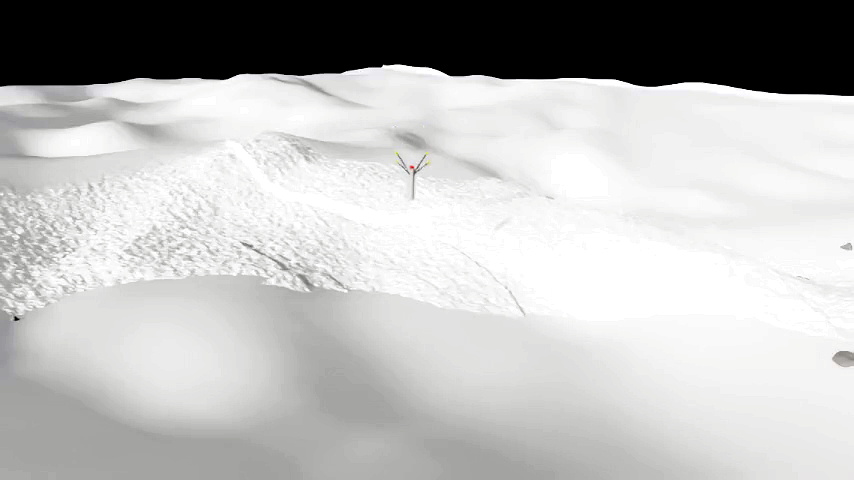
\includegraphics[width=0.86\linewidth]{sim_scene_view.png}
  \caption{Scene view captured from running the trained policy in the real
  Isaac Sim environment: the four-legged lander on cratered/rocky,
  grainy-textured lunar terrain (high-detail local patch + directional light
  for documentation; the vehicle is fully vertical as verified by simulation
  data, \texttt{up\_z} = +1.000)}
  \label{fig:scene}
\end{figure}

\begin{figure}[htb]
  \centering
  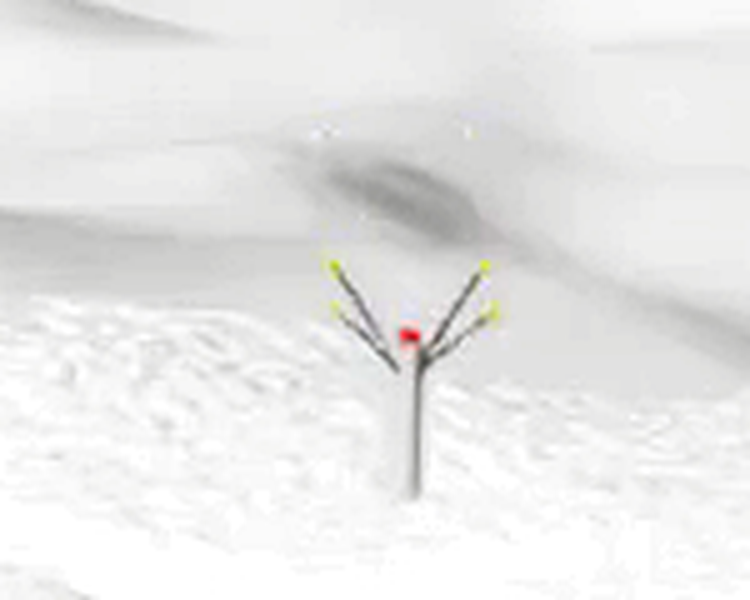
\includegraphics[width=0.52\linewidth]{sim_lander_closeup.png}
  \caption{Close-up of the same scene on the lander: the body, the tips of the
  gimbal thrust axis, and the centimetre-scale grainy texture of the ground are
  visible together}
  \label{fig:closeup}
\end{figure}

\subsection{Simulation Setup}\label{sec:setup}
This subsection collects in one place the simulation configuration shared by both the analytic (CPU) protocol and the real Isaac Lab/Isaac Sim training runs (Table~\ref{tab:simconfig}). Physics is solved GPU-parallel on NVIDIA PhysX with a fixed step of 1/120 s (120 Hz); the policy produces actions at 60 Hz with decimation = 2, and each episode lasts 20 seconds, i.e. 1200 control steps. Lunar gravity (1.62 m/s\textasciicircum{}2), a low-restitution regolith-like contact material, and 512 concurrent environment instances were held fixed across all runs.

The vehicle and actuation parameters (mass, thrust envelope, physical and policy gimbal limits, TVC actuator gains) and the SAC hyperparameters were not changed among the three blending methods. The only quantity that varies from method to method is the fine-detail fade function and its associated parameters defined in Section~\ref{sec:blend} (the last group of Table~\ref{tab:simconfig}; selected via the \texttt{ISAACLAB\_TERRAIN\_BLEND\_METHOD} environment variable). This fixing is necessary so that the differences observed in Section~\ref{sec:results} can be attributed solely to the blending method.

Because of a compute-budget constraint, the real training comparison was run with a shortened version of the full-scale (1200-iteration) configuration~--- three independent seeds per method, roughly 5.73 million environment steps per run; this scale limitation is discussed separately in Section~\ref{sec:rlprotocol} and Section~\ref{sec:rlresults}.

\begin{table}[htb]
\centering
\caption{Simulation, vehicle, RL training, and terrain-blending parameters shared by the analytic protocol and the real Isaac Lab/Isaac Sim training runs. Only the last group (blending parameters) varies from method to method.}
\label{tab:simconfig}
\footnotesize
\setlength{\tabcolsep}{4pt}
\begin{tabular}{@{}llp{0.40\linewidth}@{}}
\toprule
Group & Parameter & Value \\
\midrule
Physics / simulation & Physics engine & NVIDIA PhysX 5 (GPU pipeline) \\
 & Simulation step (dt) & 1/120 s (120 Hz) \\
 & Control frequency (decimation = 2) & 60 Hz \\
 & Episode length & 20 s (1200 control steps) \\
 & Gravity & 0, 0, -1.62 m/s\textasciicircum{}2 \\
 & Number of parallel environments & 512 \\
 & Environment spacing (\texttt{env\_spacing}) & 90 m \\
 & Physics replication & \texttt{replicate\_physics} + \texttt{clone\_in\_fabric} (on) \\
 & Friction (static / dynamic) & 0.85 / 0.65 (combine: multiply) \\
 & Restitution & 0.02 \\
Vehicle and actuation & Vehicle mass & 1.66 kg (1.63 body + gimbal linkages) \\
 & Maximum thrust & 30 N \\
 & Maximum command throttle & 0.35 (\textasciitilde{} 10.5 N effective) \\
 & Physical gimbal limit & +-25 deg (mechanical hard stop) \\
 & Policy gimbal envelope & 4 deg - 8 deg (scales with curriculum difficulty) \\
 & Thrust lever arm & 0.25 m \\
 & TVC actuator (implicit) & effort 2.5, stiffness 10, damping 0.1, armature 0.002 \\
 & Observation / action dimension & 125 / 3 \\
 & Initial altitude & 25 m (upright orientation) \\
RL training (SB3 SAC) & Policy network & MLP [384, 256, 128], ELU \\
 & Replay buffer & 1 000 000 \\
 & \texttt{learning\_starts} & 16 384 \\
 & Batch size & 1024 \\
 & Learning rate & 3e-4 \\
 & gamma / tau & 0.99 / 0.005 \\
 & \texttt{train\_freq} / \texttt{gradient\_steps} & 1 / 32 \\
 & Entropy coefficient & automatic (\texttt{target\_entropy} = -1.5) \\
 & Normalization & \texttt{normalize\_input} + \texttt{normalize\_value} on, \texttt{clip\_obs} = 10 \\
 & Comparison budget & 350 iter x 32 x 512 \textasciitilde{} 5.73 M environment steps \\
 & Seeds & 42, 7, 123 (n = 3 per method, sequential) \\
 & Device & single GPU (cuda:0) \\
Blending parameters & Transition radius (R) & 8.0 m \\
 & Method options & \texttt{smoothstep} / \texttt{gaussian} / \texttt{hybrid} (\texttt{ISAACLAB\_TERRAIN\_BLEND\_METHOD}) \\
 & Calibrated Gaussian coefficient (k) & ln(1000) \textasciitilde{} 6.9078 \\
 & Hybrid contact radius (r\_c) & 1.5 m \\
 & Hybrid switch width (w) & 0.3 m \\
 & Fine-detail amplitude range & 0.006-0.020 m \\
 & Macro height / slope scale & 0.45 m / 0.035 \\
 & Craters / rocks (per episode) & 3 / 5 \\
 & Terrain pool (size / refresh) & 15 slots / 60 assignments \\
\bottomrule
\end{tabular}
\end{table}


\subsection{Terrain Representation and Blending Functions}\label{sec:blend}
%% Hand-authored (carries the maths); build_tex.py deliberately skips this file.
The fine-detail height of the local patch is added to the global surface with
one of three candidate fade functions. In all three functions, with $r$ the
distance from the centre and $R = \texttt{terrain\_detail\_radius\_m} =
\SI{8.0}{\metre}$ the fixed transition radius, the value is forced exactly to
zero for $r \ge R$ (hard truncation); this is the key methodological
arrangement that makes the three methods comparable under the same transition
budget, and it is applied this way in the production code as well.
Figure~\ref{fig:geometry} sketches the two-layer geometry and the three fade
profiles defined below.

\paragraph{Smoothstep (compact support, default/current method).}
With $t = \operatorname{clamp}(1 - r/R,\, 0,\, 1)$,
\begin{equation}
  \mathrm{fade}_{\mathrm{ss}}(r) = t^{2}\,(3 - 2t).
  \label{eq:smoothstep}
\end{equation}
This function is already exactly zero at $r = R$; it needs no additional
truncation step, and $C^{1}$ continuity is analytically guaranteed.

\paragraph{Gaussian (infinite support, previously used method).}
\begin{equation}
  \mathrm{fade}_{\mathrm{g}}(r) = \exp\!\left(-k \left(\frac{r}{R}\right)^{2}\right).
  \label{eq:gaussian}
\end{equation}
Two values of $k$ are evaluated separately in this study: the previously used
(as-shipped) constant $k = 1.0$, and the calibrated constant proposed in this
study, $k = \ln(1000) \approx 6.9078$, which brings the Gaussian's practical
support down to roughly one part in a thousand at $R$. The
\texttt{cfg.terrain\_gaussian\_k} field in the production code uses the
calibrated constant by default; the as-shipped $k = 1.0$ was tested only in
this study's analytic/CPU comparison, as a separate variant
(\texttt{gaussian\_shipped}), to demonstrate the existing defect. For both $k$
values, the function is forced to zero externally at $r \ge R$.

\paragraph{Hybrid (proposed method).}
With the landing-gear contact-footprint radius $r_{c} =
\texttt{terrain\_hybrid\_contact\_radius\_m} = \SI{1.5}{\metre}$ and the switch
width $w = \texttt{terrain\_hybrid\_switch\_width\_m} = \SI{0.3}{\metre}$, a
smoothstep-weighted switch is defined over the interval $[\,r_{c} - w/2,\;
r_{c} + w/2\,]$. Writing $\mathrm{lo} = r_{c} - w/2$ and $\mathrm{hi} = r_{c} +
w/2$, and $u = \operatorname{clamp}\!\big((\mathrm{hi} - r)/(\mathrm{hi} -
\mathrm{lo}),\, 0,\, 1\big)$,
\begin{equation}
  \mathrm{switch}(r) = u^{2}\,(3 - 2u).
  \label{eq:switch}
\end{equation}
The final fade is then
\begin{equation}
  \mathrm{fade}_{\mathrm{hyb}}(r)
    = \mathrm{switch}(r)\,\mathrm{fade}_{\mathrm{g}}(r)
    + \big(1 - \mathrm{switch}(r)\big)\,\mathrm{fade}_{\mathrm{ss}}(r);
  \label{eq:hybrid}
\end{equation}
that is, the region near the foot contact zone is weighted mostly toward the
Gaussian, beyond it mostly toward smoothstep, and the transition between the
two functions is smoothed by a smoothstep weight that is itself $C^{1}$-smooth.
Since $\mathrm{switch}(r) = 0$ at the $r = R$ boundary, the hybrid method is
analytically identical to smoothstep at that boundary.

These three methods are integrated into the production code, selectable via the
\texttt{ISAACLAB\_TERRAIN\_BLEND\_METHOD} environment variable
(\texttt{smoothstep} \textbar{} \texttt{gaussian} \textbar{} \texttt{hybrid}),
without changing the existing default behaviour (\texttt{smoothstep}).


%% Hand-authored TikZ schematic for the Method section: the two-layer terrain
%% geometry and the three fade functions over the same transition budget.
\begin{figure}[htb]
\centering
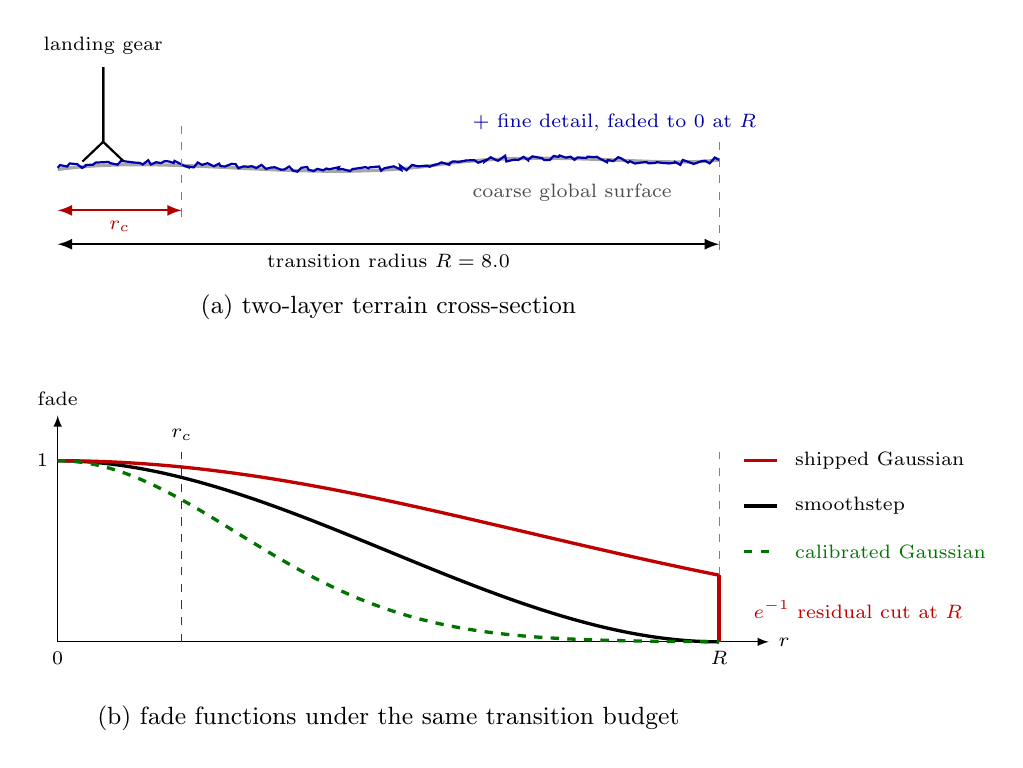
\begin{tikzpicture}[x=1.05cm, y=1cm, >=latex, font=\small]

%% ---- panel (a): two-layer cross-section --------------------------------
\begin{scope}
  % coarse global surface
  \draw[very thick, gray!70]
    (0,0) .. controls (1.4,0.20) and (3.0,-0.18) .. (4.6,0.06)
          .. controls (6.0,0.26) and (7.2,0.02) .. (8.0,0.12);
  % fine detail riding on it, faded out by R
  \draw[thick, blue!65!black, decorate,
        decoration={random steps, segment length=1.6pt, amplitude=1.1pt}]
    (0,0.02) .. controls (1.4,0.22) and (3.0,-0.16) .. (4.6,0.07)
             .. controls (6.0,0.26) and (7.2,0.02) .. (8.0,0.12);

  % landing gear feet inside the contact footprint
  \draw[thick] (0.55,1.30) -- (0.55,0.35) -- (0.30,0.10);
  \draw[thick] (0.55,1.30) -- (0.55,0.35) -- (0.80,0.10);
  \node[font=\scriptsize, anchor=south] at (0.55,1.34) {landing gear};

  % radii
  \draw[<->, thick] (0,-0.95) -- (8.0,-0.95)
    node[midway, below, font=\scriptsize] {transition radius $R=\SI{8.0}{\metre}$};
  \draw[<->, thick, red!70!black] (0,-0.52) -- (1.5,-0.52)
    node[midway, below, font=\scriptsize] {$r_c$};
  \draw[dashed, gray] (1.5,-0.60) -- (1.5,0.55);
  \draw[dashed, gray] (8.0,-1.02) -- (8.0,0.45);

  \node[anchor=west, font=\scriptsize, gray!60!black] at (4.9,-0.30)
    {coarse global surface};
  \node[anchor=west, font=\scriptsize, blue!65!black] at (4.9,0.60)
    {$+$ fine detail, faded to $0$ at $R$};
  \node[font=\small] at (4.0,-1.75) {(a) two-layer terrain cross-section};
\end{scope}

%% ---- panel (b): the three fade functions --------------------------------
\begin{scope}[yshift=-6.0cm, x=1.05cm, y=2.3cm]
  \draw[->] (0,0) -- (8.6,0) node[right, font=\scriptsize] {$r$};
  \draw[->] (0,0) -- (0,1.25) node[above, font=\scriptsize] {fade};
  \node[below, font=\scriptsize] at (0,0) {$0$};
  \node[below, font=\scriptsize] at (8.0,0) {$R$};
  \node[left, font=\scriptsize] at (0,1) {$1$};
  \draw[dashed, gray] (8.0,0) -- (8.0,1.05);

  % smoothstep: t^2(3-2t), t = 1 - r/R  -- compact support, exactly 0 at R
  \draw[very thick, black, domain=0:8, samples=90, smooth]
    plot (\x, {(1-\x/8)*(1-\x/8)*(3-2*(1-\x/8))});
  % as-shipped Gaussian k=1: never reaches 0, hard-truncated at R
  \draw[very thick, red!75!black, domain=0:8, samples=90, smooth]
    plot (\x, {exp(-1*(\x/8)^2)});
  \draw[red!75!black, very thick] (8.0,0.368) -- (8.0,0);
  % calibrated Gaussian k = ln 1000
  \draw[very thick, green!45!black, dashed, domain=0:8, samples=90, smooth]
    plot (\x, {exp(-6.9078*(\x/8)^2)});

  % contact footprint band
  \draw[red!70!black, dashed] (1.5,0) -- (1.5,1.05);
  \node[font=\scriptsize, anchor=south] at (1.5,1.06) {$r_c$};

  % curve labels live in a key to the right of the plot, clear of every curve
  \node[font=\scriptsize, red!75!black, anchor=west] at (8.3,0.18)
    {$e^{-1}$ residual cut at $R$};
  \draw[very thick, red!75!black] (8.3,1.00) -- (8.7,1.00);
  \node[font=\scriptsize, anchor=west] at (8.8,1.00) {shipped Gaussian};
  \draw[very thick, black] (8.3,0.75) -- (8.7,0.75);
  \node[font=\scriptsize, anchor=west] at (8.8,0.75) {smoothstep};
  \draw[very thick, green!45!black, dashed] (8.3,0.50) -- (8.7,0.50);
  \node[font=\scriptsize, anchor=west, green!45!black] at (8.8,0.50) {calibrated Gaussian};
  \node[font=\small] at (4.0,-0.42)
    {(b) fade functions under the same transition budget};
\end{scope}

\end{tikzpicture}
\caption{Geometry of the blending problem. (a) The fine-detail local patch is
faded into the coarse global surface inside a fixed transition radius $R$; the
landing gear contacts the surface within the much smaller footprint radius
$r_c$. (b) The three candidate fade functions on the same budget. Smoothstep
has compact support and reaches exactly zero at $R$; the as-shipped Gaussian
($k=1$) still carries roughly $e^{-1}\approx\SI{37}{\percent}$ of its amplitude
at $R$, so hard truncation there leaves the seam this study measures; the
calibrated Gaussian ($k=\ln 1000$) decays to about one part in a thousand by
$R$. The hybrid follows the Gaussian inside $r_c$ and smoothstep beyond it, and
is analytically identical to smoothstep at the boundary}
\label{fig:geometry}
\end{figure}


\subsection{Analytic (CPU) Evaluation Protocol}\label{sec:analytic}
The analytic evaluation was carried out, with no Isaac Lab/torch dependency, on a one-to-one NumPy port of the formulas in the production code, along two independent tracks: (i) a mesh track, which generates the actual triangle mesh and measures vertex count and time; (ii) an analytic track, which queries the height field directly as a continuous function. Having the two tracks validate each other was used to show that the findings are not an artefact specific to mesh discretization.

The continuity metrics were computed with finite differences: C0 (height) continuity is defined as the absolute value of the height difference between points immediately on either side of the transition boundary (spatial epsilon = 0.05 m); C1 (slope) continuity as the angular difference of the local gradient at the same points (gradient epsilon = 0.02 m). Measurements were taken over 720 angular samples, and both the maximum and the RMS (root mean square) values are reported. In the initial measurements, the measurement made on the combined (global + local) height was seen to mix with the variation of the natural terrain slope over the epsilon interval and to suppress the actual seam signal; for this reason a "detail-only" measurement mode was defined, isolating only the faded fine-detail component (fade(r) * fine\_detail(x,y)), and this was adopted as the study's headline metric; the measurement on the combined surface was retained as a secondary/realistic reference.

Memory cost was estimated separately for the two-mesh (literal, separate global and local meshes) and single-grid (baked, one combined mesh) accounting schemes, under the assumption of 32 bytes per vertex and a 2x multiplier for the collision mesh. Query throughput was also measured: the cost in microseconds of the pure fade formula (fade-only, isolated from terrain sampling), under the assumption of 512 environments and 64 global + 24 local + 4 fine-detail queries per environment (92 queries/environment in total).

The main comparison was repeated over thirty independent random seeds for the four method variants (\texttt{smoothstep}, as-shipped Gaussian, calibrated Gaussian, \texttt{hybrid}); statistical significance was assessed with the Wilcoxon signed-rank test on the per-seed log10 ratio differences (this test was preferred over parametric tests because in some comparisons~--- e.g. \texttt{hybrid} versus \texttt{smoothstep}, which are analytically identical at r = R~--- the difference distribution converges to near-zero variance and parametric effect-size measures such as Cohen's d degenerate).

The robustness of the findings was tested with four separate ablation analyses: (i) a contact-radius (rc) sweep over 1.0-4.0 m; (ii) a switch-width (w) sweep over 0.05-2.0 m; (iii) a transition-radius (R) sweep over 4-16 m, to test the scale-invariance of the defect; (iv) a grid-resolution sweep over roughly 0.31-1.27 m grid spacing, estimating the empirical convergence order by log-log linear regression.


\subsection{Reinforcement Learning Method (MDP Formulation and SAC)}\label{sec:rl}
This subsection defines the learning problem on which the three blending methods are compared in real simulation, and the reinforcement learning (RL) method used to solve that problem. The algorithm and hyperparameter configuration were never changed among the three methods (see Table~\ref{tab:simconfig}); this subsection therefore describes the "fixed" component of the comparison.

Formulation of the task as a Markov decision process (MDP). The landing task is treated as a discrete-time MDP (S, A, P, r, gamma). The state observation is 125-dimensional and consists of the following component groups: position relative to the target, the body's linear and angular velocity in the world frame, the orientation quaternion, the instantaneous thrust acceleration transformed into the body frame, the minimum foot-to-ground clearance, the current and previous action vectors, local terrain slope/roughness metrics around the target, a 64-ray LiDAR profile scanning the surroundings of the body, a 24-point local terrain height scan below the target, and (noise-added) sensor features derived from IMU/altimeter readings. All components are scaled to the [-1, 1] or [0, 1] band by their physical ranges and clipped against outliers with \texttt{clip\_obs} = 10. The action space is 3-dimensional and continuous, [-1, 1]\textasciicircum{}3: the first component is the main thrust command and is effectively mapped to the 0-0.35 throttle range (roughly 10.5 N); the second and third components are the two-axis gimbal (thrust-vectoring) angle, and the envelope the policy can command scales with curriculum difficulty between +-4 deg and +-8 deg (the mechanical hard stop is at +-25 deg). The transition dynamics P are the physics simulation solved on NVIDIA PhysX at 120 Hz; the policy produces actions at 60 Hz with decimation = 2, and each episode lasts 20 seconds, i.e. 1200 control steps. The discount factor is gamma = 0.99.

Reward function. The reward is the sum of dense and terminal terms: r = xy\_progress + altitude\_progress + stability + velocity + guidance + control + terrain + time + terminal. Each dense term is defined either as a progress difference between two consecutive steps or as a per-second cost; this design prevents an early crash from becoming attractive merely because it stops the step penalties. The largest weights concentrate on horizontal approach to the target (+12.0 per unit decrease in distance), deviation from the desired vertical descent speed (-8.0), and guidance deviation from the desired thrust-acceleration profile (-6.0); the remaining dense terms penalize tilt relative to the local terrain normal, angular velocity, fuel/gimbal usage, action smoothness, and the fit of the footprint to the terrain. The terminal term is paid only once per episode and depends on the landing classification: soft landing +300, harsh landing -220 (with a correction between 0 and +160 depending on landing quality), out-of-bounds/crash -220, timeout -150. The classification is made according to foot contact, the vehicle's residual tilt relative to the local terrain normal (not world-vertical), and speed/footprint-fit thresholds. The detailed rationale for the reward weights is documented in the source comments of the production code; it was not changed during this study's comparison.

Soft Actor-Critic (SAC). The policy was learned with SAC, an off-policy actor-critic algorithm with a maximum-entropy objective \citep{haarnoja2018}. SAC optimizes not only the expected reward but an objective regularized by the policy's entropy: pi* = argmax\_pi sum\_t E[r(s\_t, a\_t) + alpha H(pi(. | s\_t))]. The entropy term H here encourages the agent to remain stochastic even as it converges toward high reward; in a contact-rich landing problem with many local optima, this delays the policy prematurely turning deterministic and locking into a weak behaviour (premature convergence). SAC's sample efficiency~--- obtained by reusing a replay buffer repeatedly~--- and its relative robustness to hyperparameters are the reasons this algorithm was chosen for a physics simulation that is expensive even when GPU-parallel. In practice, two independent Q-critic networks (clipped double-Q, which reduces value overestimation bias), target networks updated slowly by Polyak averaging (tau = 0.005), and automatic tuning of the temperature coefficient alpha by anchoring it to a target entropy are used; alpha is learned during training by the gradient of the objective J(alpha) = E[-alpha (log pi(a | s) + H\_target)]. Concretely, the SAC implementation of the Stable-Baselines3 library was used \citep{raffin2021}.

Network architecture and hyperparameters. The actor and critic networks are multi-layer perceptrons (MLPs) with hidden layer sizes [384, 256, 128] and ELU activation. The replay buffer has a capacity of 10\textasciicircum{}6 transitions; the first 16,384 transitions are for buffer filling only (\texttt{learning\_starts}). The batch size is 1024, the learning rate is 3 x 10\textasciicircum{}-4 (Adam), gamma = 0.99, tau = 0.005. Each vectorized environment step produces 512 transitions, and 32 gradient steps are taken per vector step (\texttt{train\_freq} = 1, \texttt{gradient\_steps} = 32): a single update per vector step markedly under-trains SAC, whereas 32 updates provide enough policy updates for the curriculum while preserving parallel-simulation throughput. Observations and value targets are normalized with running statistics (\texttt{normalize\_input} and \texttt{normalize\_value} on). This normalization solves a scale problem: because terminal rewards are on the order of +300/-220 while dense terms can accumulate to over +-1000 per episode, without normalization the critic/value targets dominate the SAC update scale, and the temperature coefficient collapses from 0.85 to 0.025 in about 50 thousand steps, turning the actor deterministic before it has learned anything meaningful. For the same reason the target entropy is set to -1.5 instead of the default -action\_dim = -3; this value leaves markedly more exploration in the early curriculum phases. All of these hyperparameters are listed in Table~\ref{tab:simconfig} and are fixed across the three blending methods.

Curriculum. Training is carried out within a curriculum in which the spawn distance, the target distance, and the gimbal authority the policy can command increase together. The difficulty level is a scalar in [0.05, 1.0]; for each episode the effective difficulty is sampled as torch.rand() x level, i.e. even at the highest level the episodes in a batch are distributed from easy to hard. If the rolling-window success rate exceeds the threshold curriculum\_success\_threshold = 0.35, the level increases by 0.05; if it falls below half the threshold, it decreases by 0.05. The window size scales with the number of environments (at least 4 x num\_envs completed episodes): a fixed, small window fills with only a few resets at high environment counts, causing difficulty to race toward \textasciitilde{}1.0 much faster than the policy has actually learned, and then a measurable performance regression (a training collapse documented in the README). Similarly, since the gimbal envelope saturating in the first 30\% of the curriculum produced a reproducible collapse when the hardest episodes of a batch suddenly hit the harsh 8 deg gimbal saturation, this envelope is spread across the entire curriculum range (curriculum\_full\_gimbal\_difficulty = 1.0). These two arrangements are common to all of the comparison runs described below in Section~\ref{sec:rlprotocol}.


\subsection{Isaac Lab/Isaac Sim Training Protocol}\label{sec:rlprotocol}
After the analytic evaluation, the three methods (\texttt{smoothstep}, calibrated Gaussian, \texttt{hybrid}) were compared in a real Isaac Lab/Isaac Sim training environment. This forms the centre of the study's novelty: the comparison was carried out not as an abstract numerical experiment but with a SAC training loop running inside a GPU-parallel PhysX physics simulation, on real cratered/sloped lunar terrain.

Each method, selected via the \texttt{ISAACLAB\_TERRAIN\_BLEND\_METHOD} environment variable, was trained on the same hardware (single machine, single GPU), with the same SAC configuration defined in Section~\ref{sec:rl} (sb3\_sac\_cfg.yaml), and sequentially rather than concurrently, to avoid GPU/VRAM contention. Each run lasted 5,734,400 environment steps (roughly 350 iterations); this is a shortened but still meaningful-signal version of the full-scale (1200-iteration) configuration, reduced because of a compute-budget constraint, and this is a scale limitation that must be stated explicitly.

The initial measurement was made as a single run per method, with the default seed in the SAC agent's configuration file (seed = 42). Considering that this single-run design is exactly the kind of pitfall \citet{henderson2018} warn about, the study was extended with two additional independent seeds (seed = 7 and seed = 123), yielding a total of three independent runs (n = 3) per method~--- the ISAACLAB\_SEED environment variable was added to the production code for this purpose. Because of the inherent nondeterminism of GPU-parallel PhysX physics simulation (thread scheduling, floating-point reduction order) and the timing dependence of the terrain pool's background CPU generation process, even two runs with the same seed are not bit-equivalent repeats of each other; the three seeds therefore sample this system-level nondeterminism in addition to the variance due to agent initialization.

Training metrics (success rate, timeout rate, harsh-landing rate, curriculum difficulty, entropy coefficient, xy-progress reward) were logged via TensorBoard, and the event files were parsed with tensorboard.backend.event\_processing.EventAccumulator. For each (method, seed) run, the final performance was reduced to a SINGLE summary value by averaging the logged points in that run's final ten-percent window; comparisons among methods were made on these three independent summary values (as an independent sample) with the Mann-Whitney U test and a 5000-replicate bootstrap 95\% confidence interval. This is the statistically correct unit, avoiding the use of autocorrelated (non-independent) points within a single run as a pseudo-independent sample (pseudoreplication); however, statistical power with n = 3 is low, and this point is emphasized explicitly in Section~\ref{sec:rlresults} and Section~\ref{sec:discussion}.


\section{Results}\label{sec:results}
This section presents the boundary-continuity and computational-cost findings, then the results of the four ablation analyses, and finally the results of the real Isaac Sim training comparison. No method is repeated; the data/experimental-design details are left to Section~\ref{sec:method}.


\subsection{Boundary Continuity and Computational Cost}\label{sec:continuity}
Table~\ref{tab:continuity} summarizes, as a ratio relative to \texttt{smoothstep}, the headline continuity measurements aggregated over thirty seeds and isolating only the faded fine-detail component. The as-shipped Gaussian (\texttt{gaussian\_shipped}, k = 1.0) produces on average 3192 times worse C0 (height) continuity and 535 times worse C1 (slope) continuity than \texttt{smoothstep}; both differences are extremely significant by the Wilcoxon signed-rank test (p = 1.86e-09, n = 30). The calibrated Gaussian (k = ln(1000)) largely removes this defect but still leaves measurably higher residual error than \texttt{smoothstep} (roughly 9.3x on C0, roughly 1.6x on C1). The \texttt{hybrid} method, being analytically identical to \texttt{smoothstep} at the r = R boundary (switch(R) = 0), showed zero difference on all thirty seeds; this is not a measurement result but an expected consequence of the method's definition.

\begin{table}[htb]
\centering
\caption{Boundary continuity ratios relative to smoothstep, aggregated over thirty seeds, isolating only the fine-detail component. C0 is the RMS boundary height error and C1 the RMS slope error; both columns are ratios to the smoothstep reference. p is the Wilcoxon signed-rank p value.}
\label{tab:continuity}
\footnotesize
\setlength{\tabcolsep}{4pt}
\begin{tabular}{@{}lrrrr@{}}
\toprule
Method & C0 ratio & C1 ratio & Wilcoxon p & n \\
\midrule
\texttt{smoothstep} (reference) & 1.0 & 1.0 & - & 30 \\
\texttt{gaussian\_shipped} (k=1.0) & 3192x & 535x & 1.86e-09 & 30 \\
\texttt{gaussian\_calibrated} (k=ln(1000)) & 9.3x & 1.6x & 1.86e-09 & 30 \\
\texttt{hybrid} & 1.0 (identical) & 1.0 (identical) & n/a (analytically identical) & 30 \\
\bottomrule
\end{tabular}
\end{table}


Figure~\ref{fig:radial} shows the combined (macro + fine detail) height cross-section of the four method variants. At this scale the four curves almost exactly overlap, because the fine-detail amplitude (on the order of centimetres) is very small compared with the macro terrain scale (on the order of metres); the order-of-magnitude differences reported in Table~\ref{tab:continuity} cannot be discerned by eye at this visual scale. This directly demonstrates why the "detail-only" isolation step defined in Section~\ref{sec:analytic} is necessary: the seam defect emerges only when the fine-detail component is separated out.

\begin{figure}[htb]
  \centering
  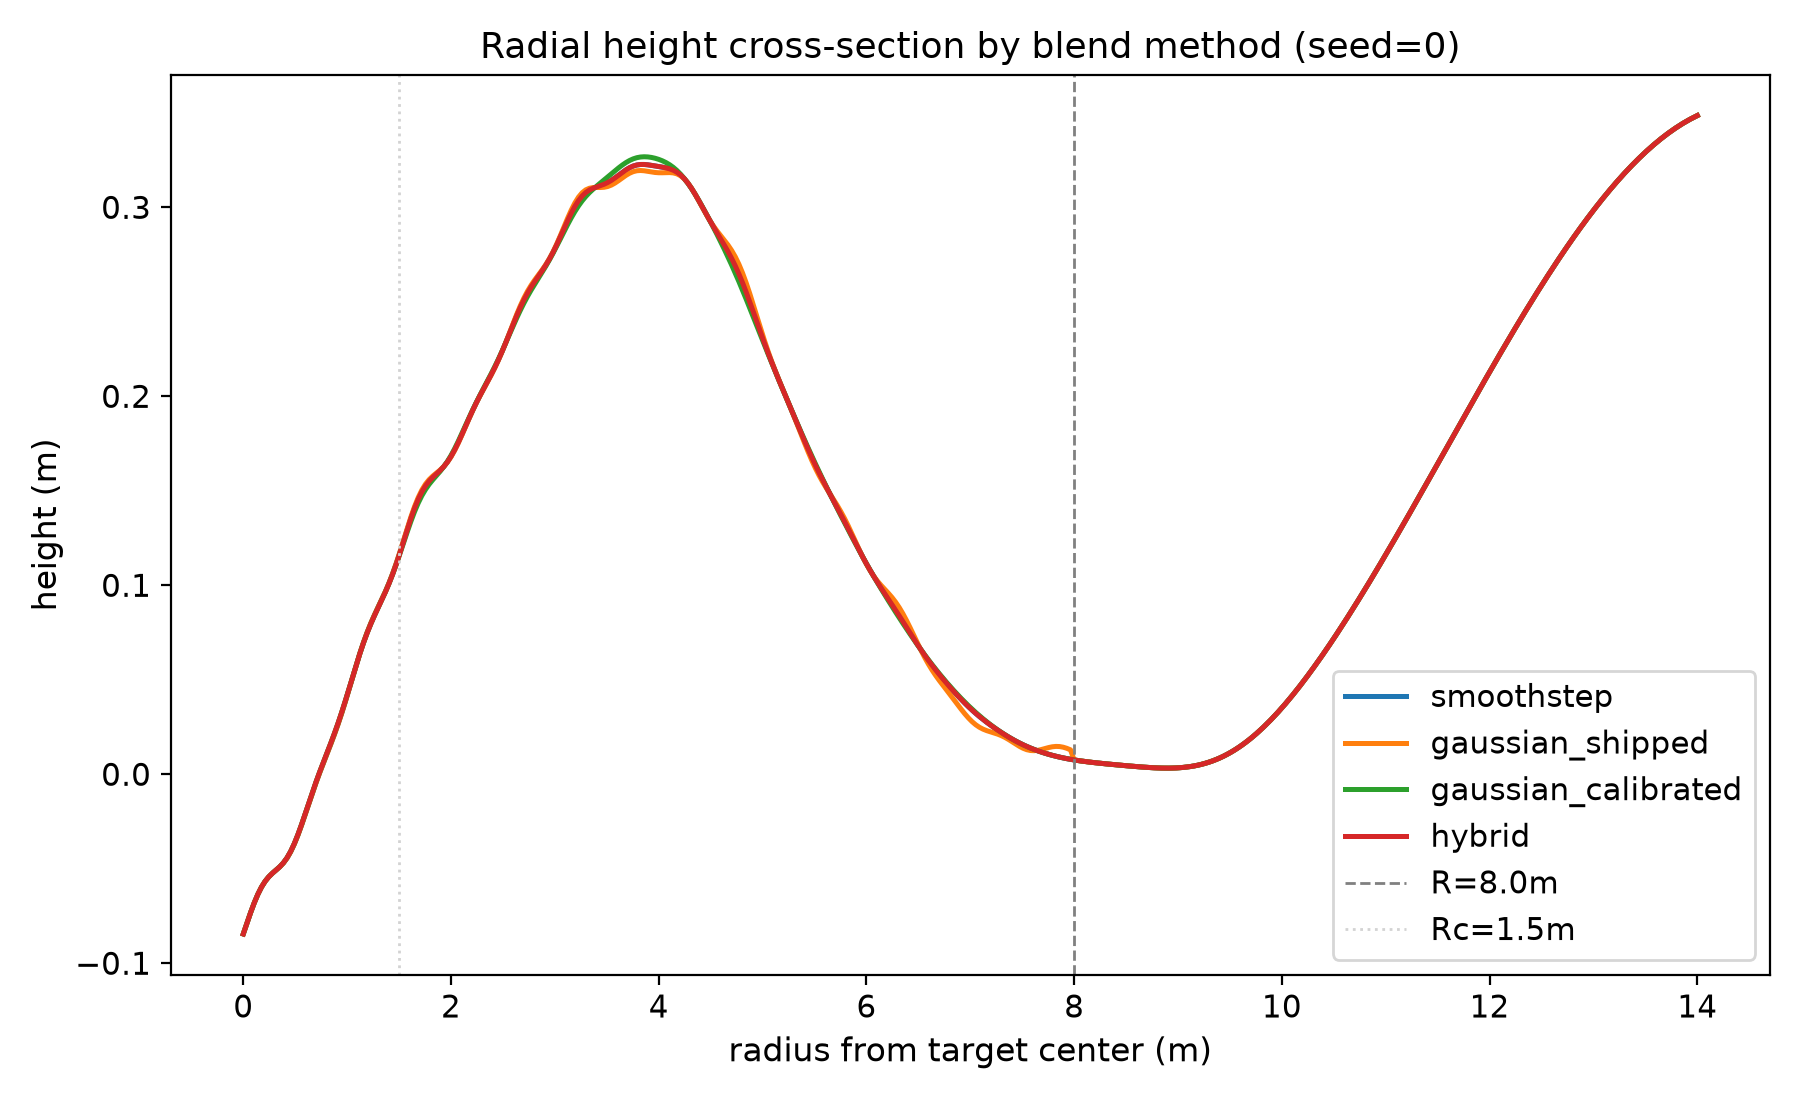
\includegraphics[width=0.92\linewidth]{radial_profile.png}
  \caption{Radial fade profile of the three blending methods}
  \label{fig:radial}
\end{figure}

Table~\ref{tab:fadecost} shows the computational cost, in microseconds, of the fade formula itself (isolated from terrain sampling). Smoothstep has the lowest cost (93.1 microseconds); the Gaussian variants (as-shipped and calibrated) have a similar, mid-level cost (roughly 149-150 microseconds); the \texttt{hybrid} method has the highest cost (407.8 microseconds, roughly 4.3 times that of \texttt{smoothstep}), because it computes both the Gaussian and the \texttt{smoothstep} branches as well as the switch weight on every query.

\begin{table}[htb]
\centering
\caption{Per-query computational cost of the fade formula.}
\label{tab:fadecost}
\footnotesize
\setlength{\tabcolsep}{4pt}
\begin{tabular}{@{}lr@{}}
\toprule
Method & Cost (us/query) \\
\midrule
\texttt{smoothstep} & 93.12 \\
\texttt{gaussian\_shipped} & 148.84 \\
\texttt{gaussian\_calibrated} & 149.61 \\
\texttt{hybrid} & 407.83 \\
\bottomrule
\end{tabular}
\end{table}


Figure~\ref{fig:contcmp} visualizes the analytic and mesh-track continuity measurements of Table~\ref{tab:continuity} as a bar chart per method; that \texttt{gaussian\_shipped} has an error bar orders of magnitude higher than the other three methods in all four panels also visually confirms the magnitude difference reported in the table.

\begin{figure}[htb]
  \centering
  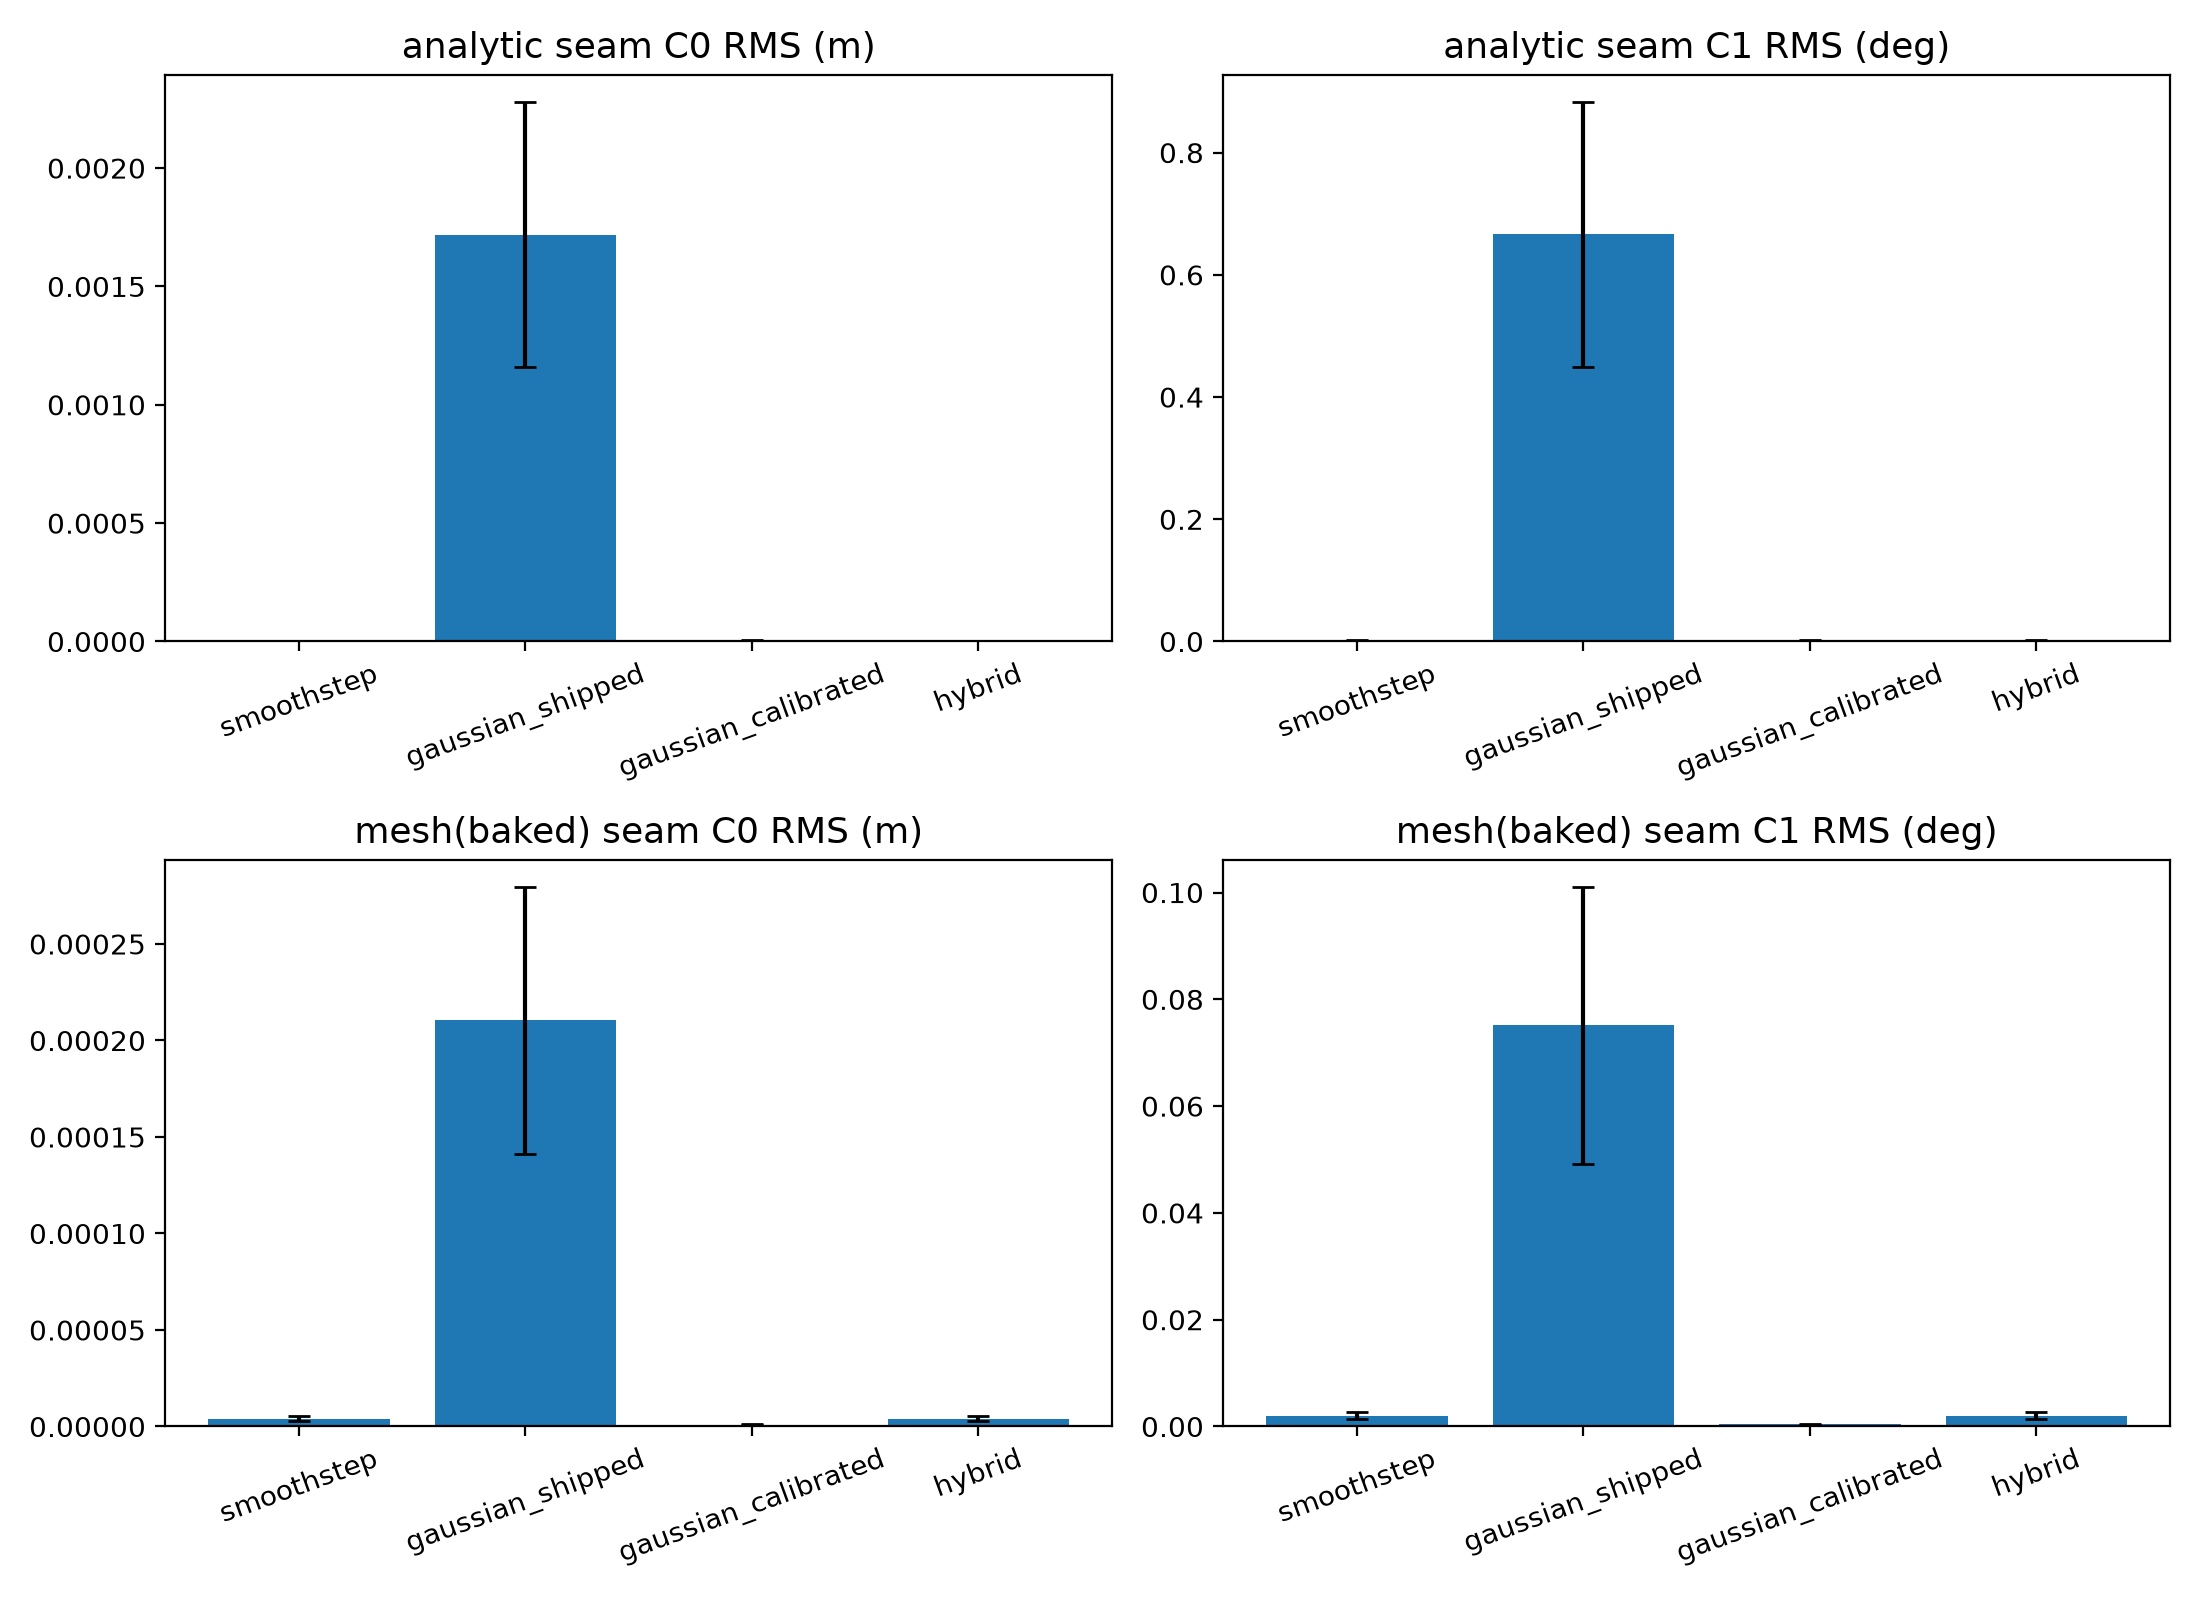
\includegraphics[width=0.92\linewidth]{continuity_comparison.png}
  \caption{Cross-method comparison of C0/C1 boundary continuity}
  \label{fig:contcmp}
\end{figure}

Table~\ref{tab:vram} shows the memory estimate for the two mesh accounting schemes; this estimate depends only on the mesh geometry (vertex count), and the shape of the blending method has no measurable effect on VRAM~--- the real VRAM lever is the mesh topology choice (two-mesh versus single-grid), not the choice of blending function.

\begin{table}[htb]
\centering
\caption{Estimated VRAM usage by mesh accounting scheme.}
\label{tab:vram}
\footnotesize
\setlength{\tabcolsep}{4pt}
\begin{tabular}{@{}lr@{}}
\toprule
Mesh accounting scheme & Estimated memory (MB) \\
\midrule
Two-mesh (literal: separate global + local meshes) & 5.24 \\
Single-grid (baked: one combined mesh) & 1.05 \\
\bottomrule
\end{tabular}
\end{table}


Figure~\ref{fig:costcmp} combines the cost measures of Table~\ref{tab:fadecost} and Table~\ref{tab:vram} into a single view: the mesh-track generation time and the analytic-track query throughput are relatively close across methods, while the \texttt{hybrid}'s marked jump in fade-only cost and the fact that all four methods share the same VRAM footprint can be seen together in the same set of plots.

\begin{figure}[htb]
  \centering
  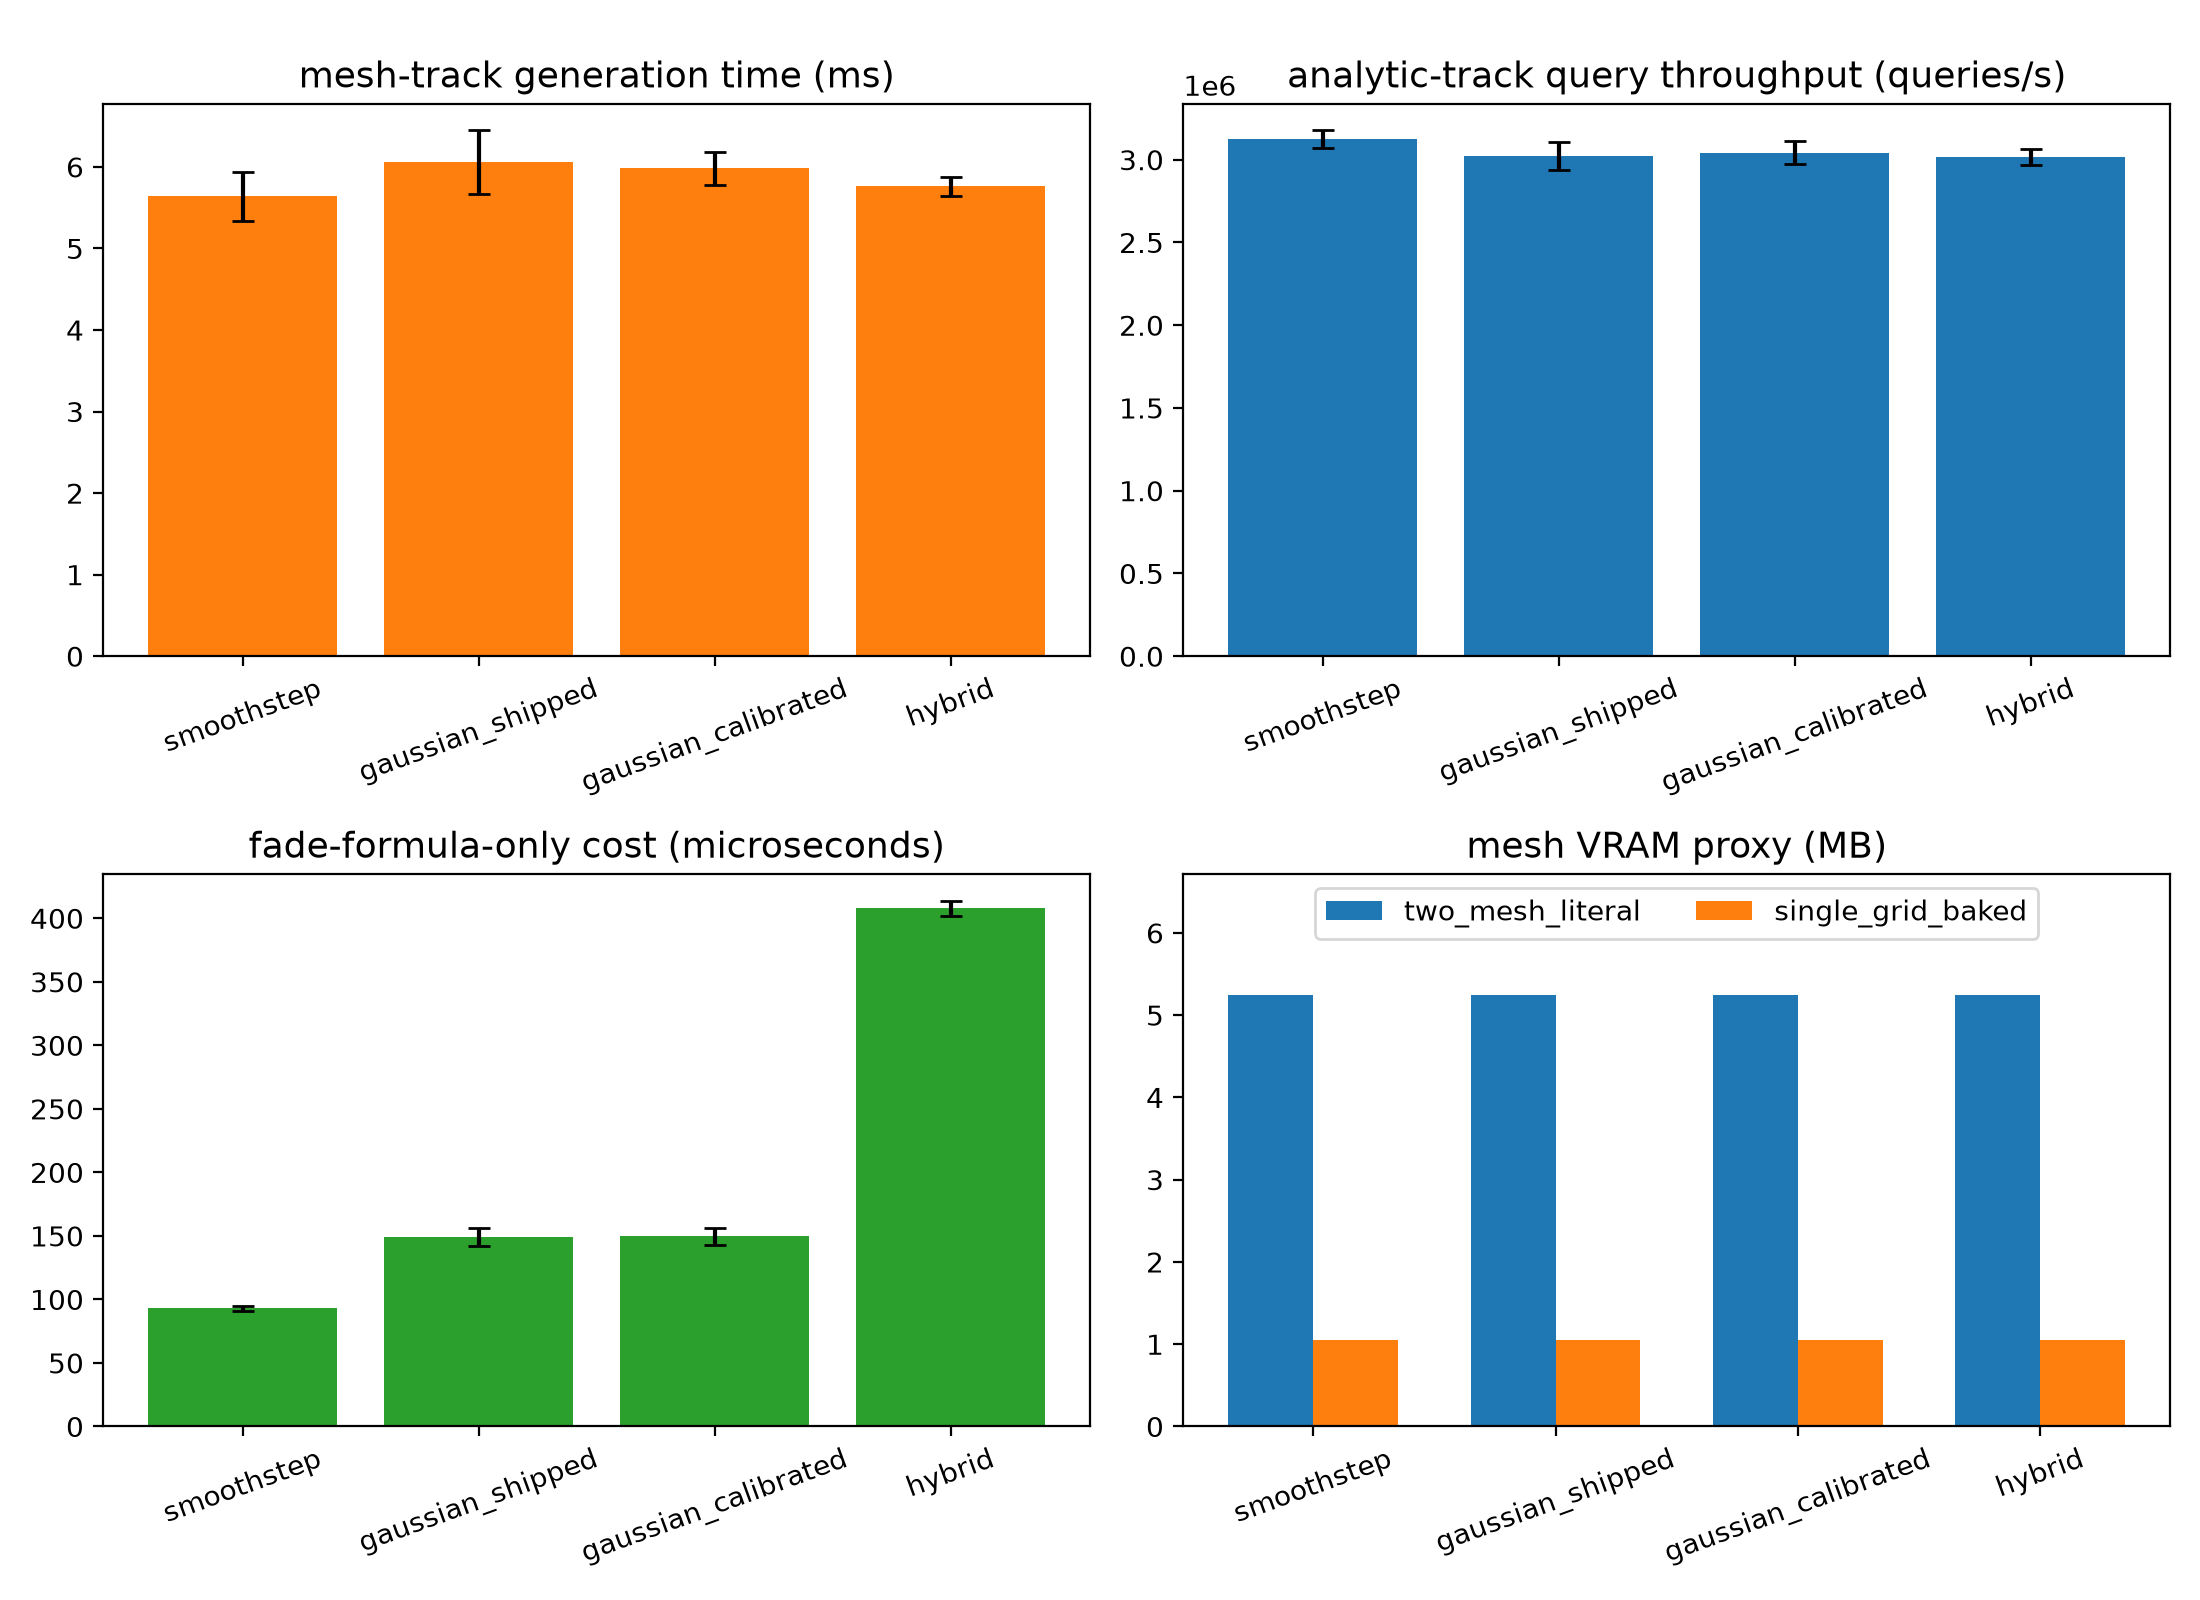
\includegraphics[width=0.92\linewidth]{cost_comparison.png}
  \caption{Cross-method comparison of computational cost}
  \label{fig:costcmp}
\end{figure}

\subsection{Ablation Analyses}\label{sec:ablation}
This section presents four separate ablation analyses that test the robustness of the proposed \texttt{hybrid} method against its four design parameters (contact radius, switch width, transition radius, grid resolution).


In the contact-radius (rc) sweep of the \texttt{hybrid} method (1.0-4.0 m; Figure~\ref{fig:rcsweep}), the C0 discontinuity at the switch's own internal transition boundary (r = rc) stayed below 3e-4 m at all rc values, and the fade cost stayed constant regardless of rc (roughly 755-793 microseconds); this confirms that the cost stems not from where the switch is located but from both branches being computed in every case.

\begin{figure}[htb]
  \centering
  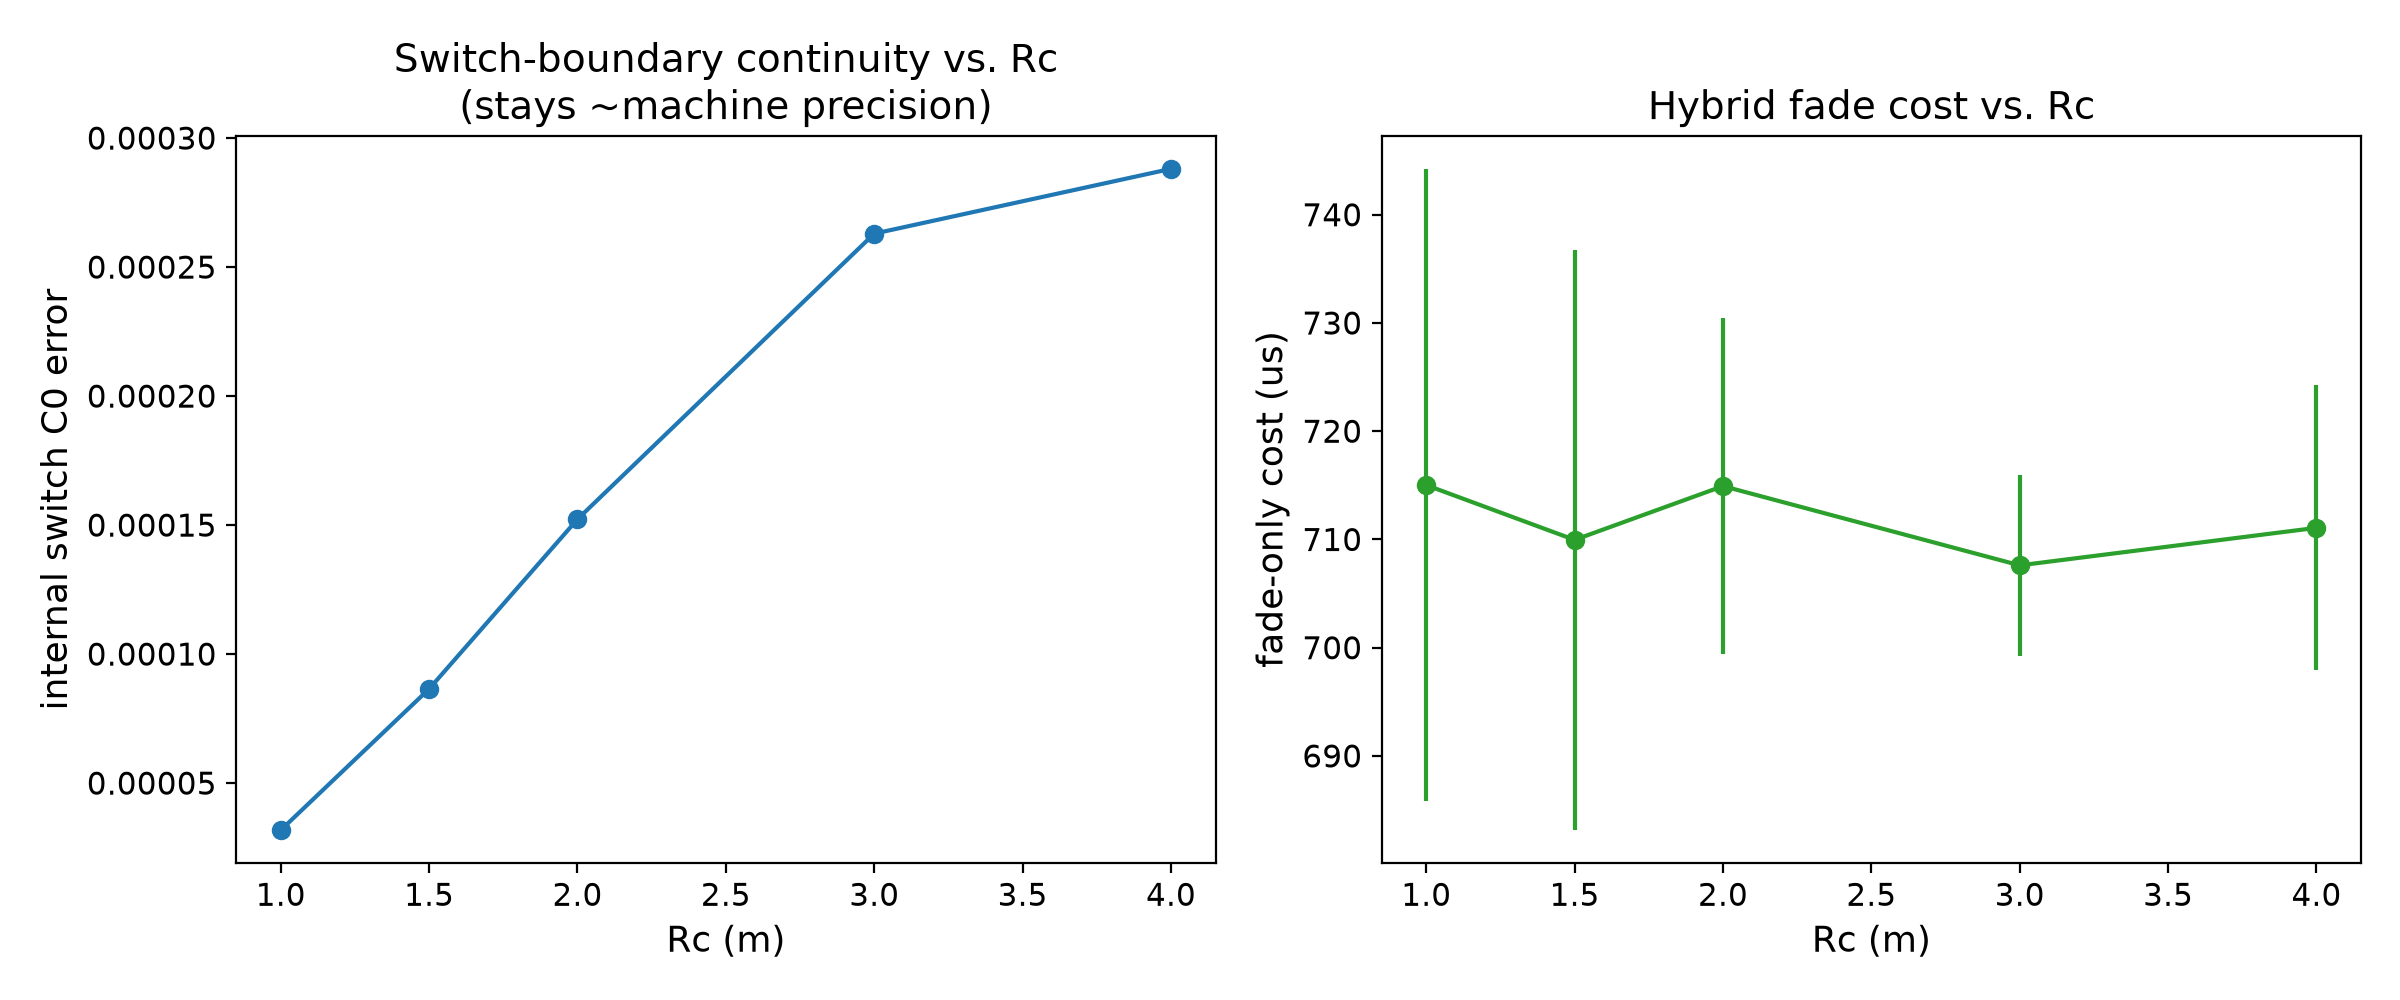
\includegraphics[width=0.92\linewidth]{rc_sweep.png}
  \caption{Contact-radius ($r_c$) sweep: switch internal continuity and cost}
  \label{fig:rcsweep}
\end{figure}

In the switch-width (w) sweep (0.05-2.0 m; Figure~\ref{fig:wsweep}), the switch's internal continuity improved steadily from 7.03e-4 m at w = 0.05 m to 1.74e-7 m at w = 1.0 m, but worsened slightly at w = 2.0 m (1.83e-5 m); this suggests that once the switch width approaches magnitudes near the contact radius, the switch begins to distort its own local curvature, and it shows that w roughly in the 0.3-1.0 m range is a suitable default for internal continuity near machine precision; the w = 0.3 m used in the production configuration provides a deliberate safety margin within this range.

\begin{figure}[htb]
  \centering
  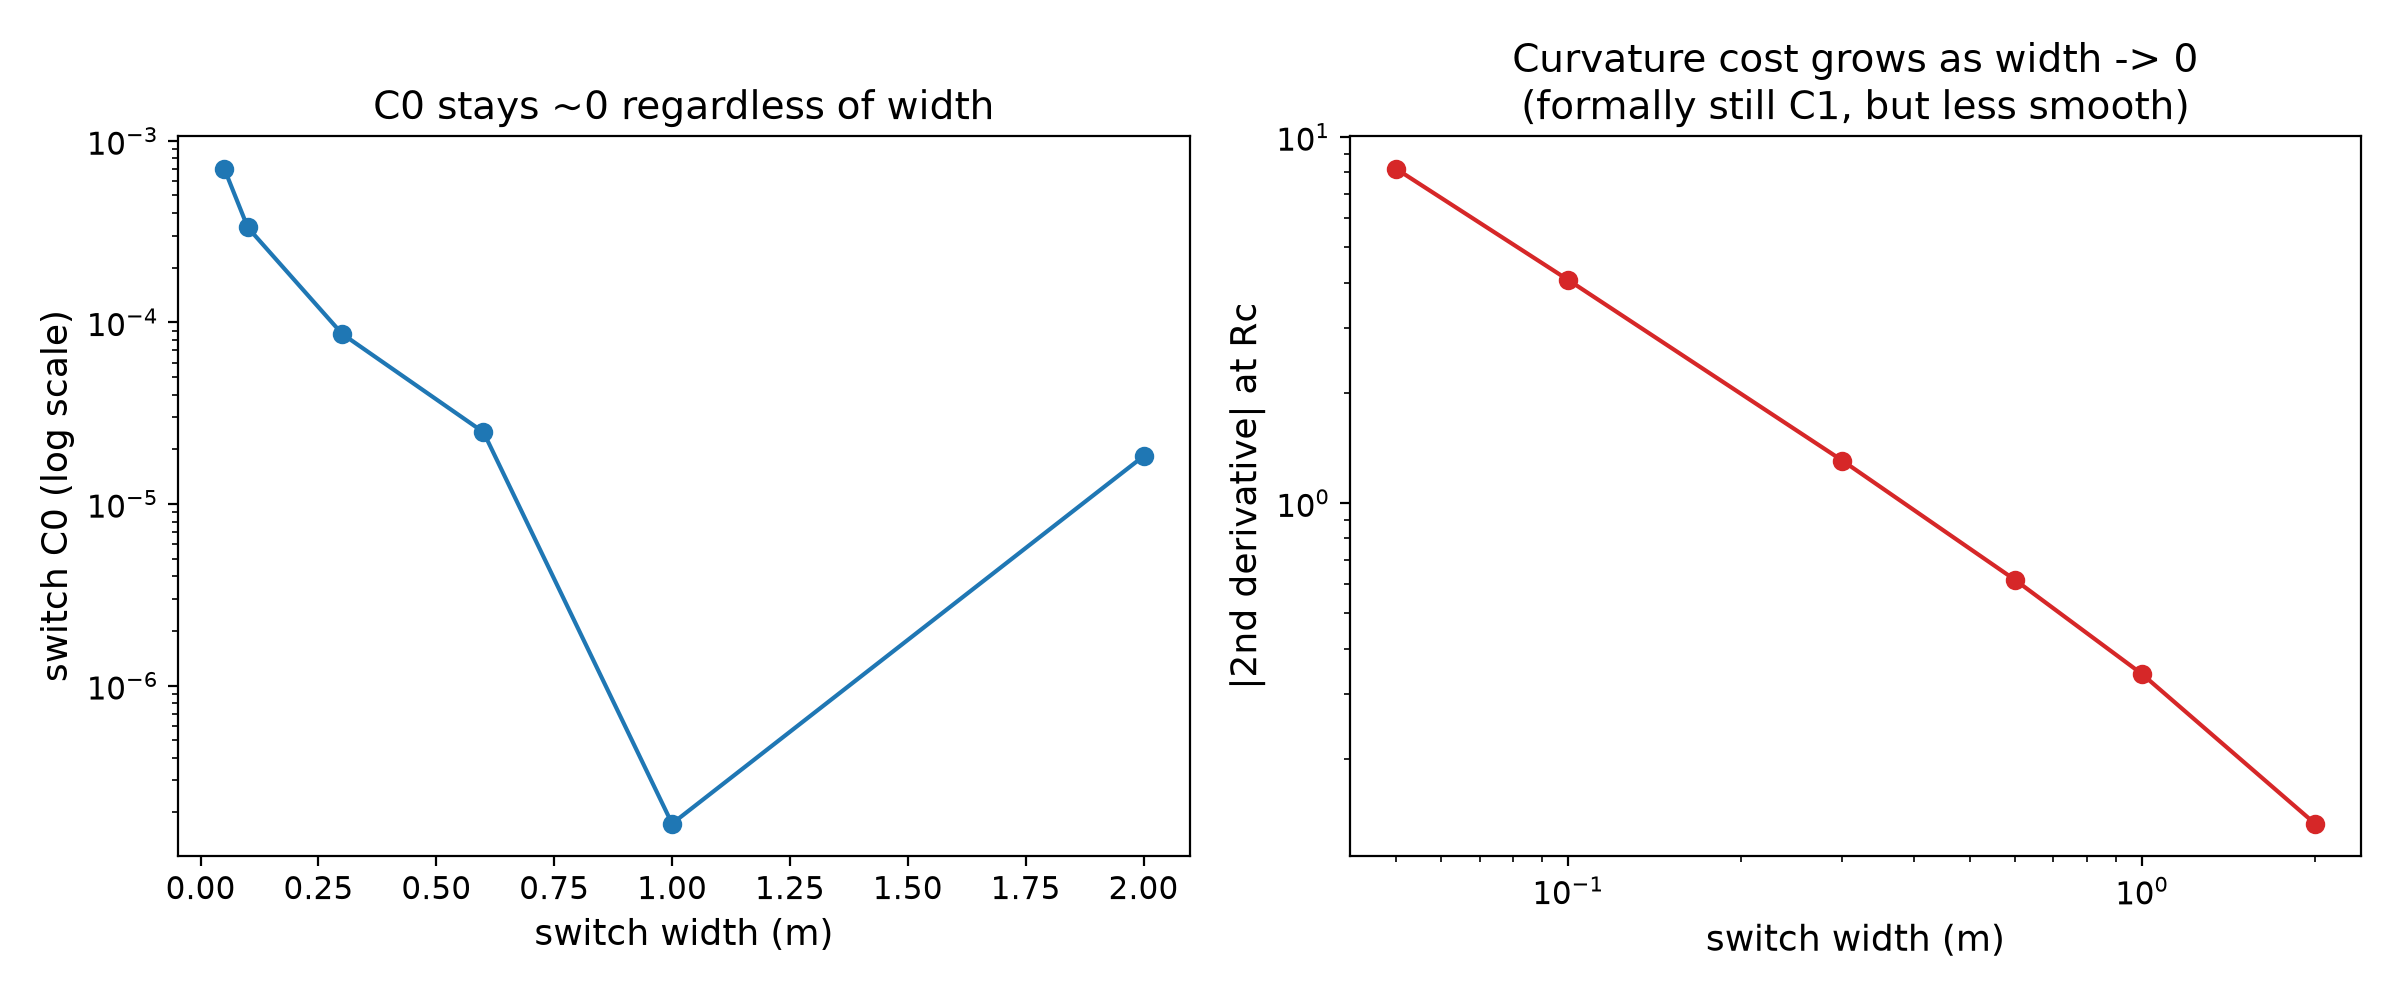
\includegraphics[width=0.92\linewidth]{switch_width_sweep.png}
  \caption{Switch-width ($w$) sweep: internal continuity}
  \label{fig:wsweep}
\end{figure}

In the radius sweep performed to test whether this defect is independent of the transition radius (R = 4, 6, 8, 12, 16 m; Figure~\ref{fig:rsweep}), the as-shipped Gaussian's C0 (RMS) error stays almost constant (between roughly 1.68e-3 and 1.76e-3 m), i.e. the error does not shrink as the transition radius grows; by contrast, the error of \texttt{smoothstep} and the calibrated Gaussian decreases steadily as the radius grows (as the curvature decreases), as expected. This shows that the as-shipped Gaussian's defect is not a discretization error but a scale-invariant structural property, independent of the transition radius.

\begin{figure}[htb]
  \centering
  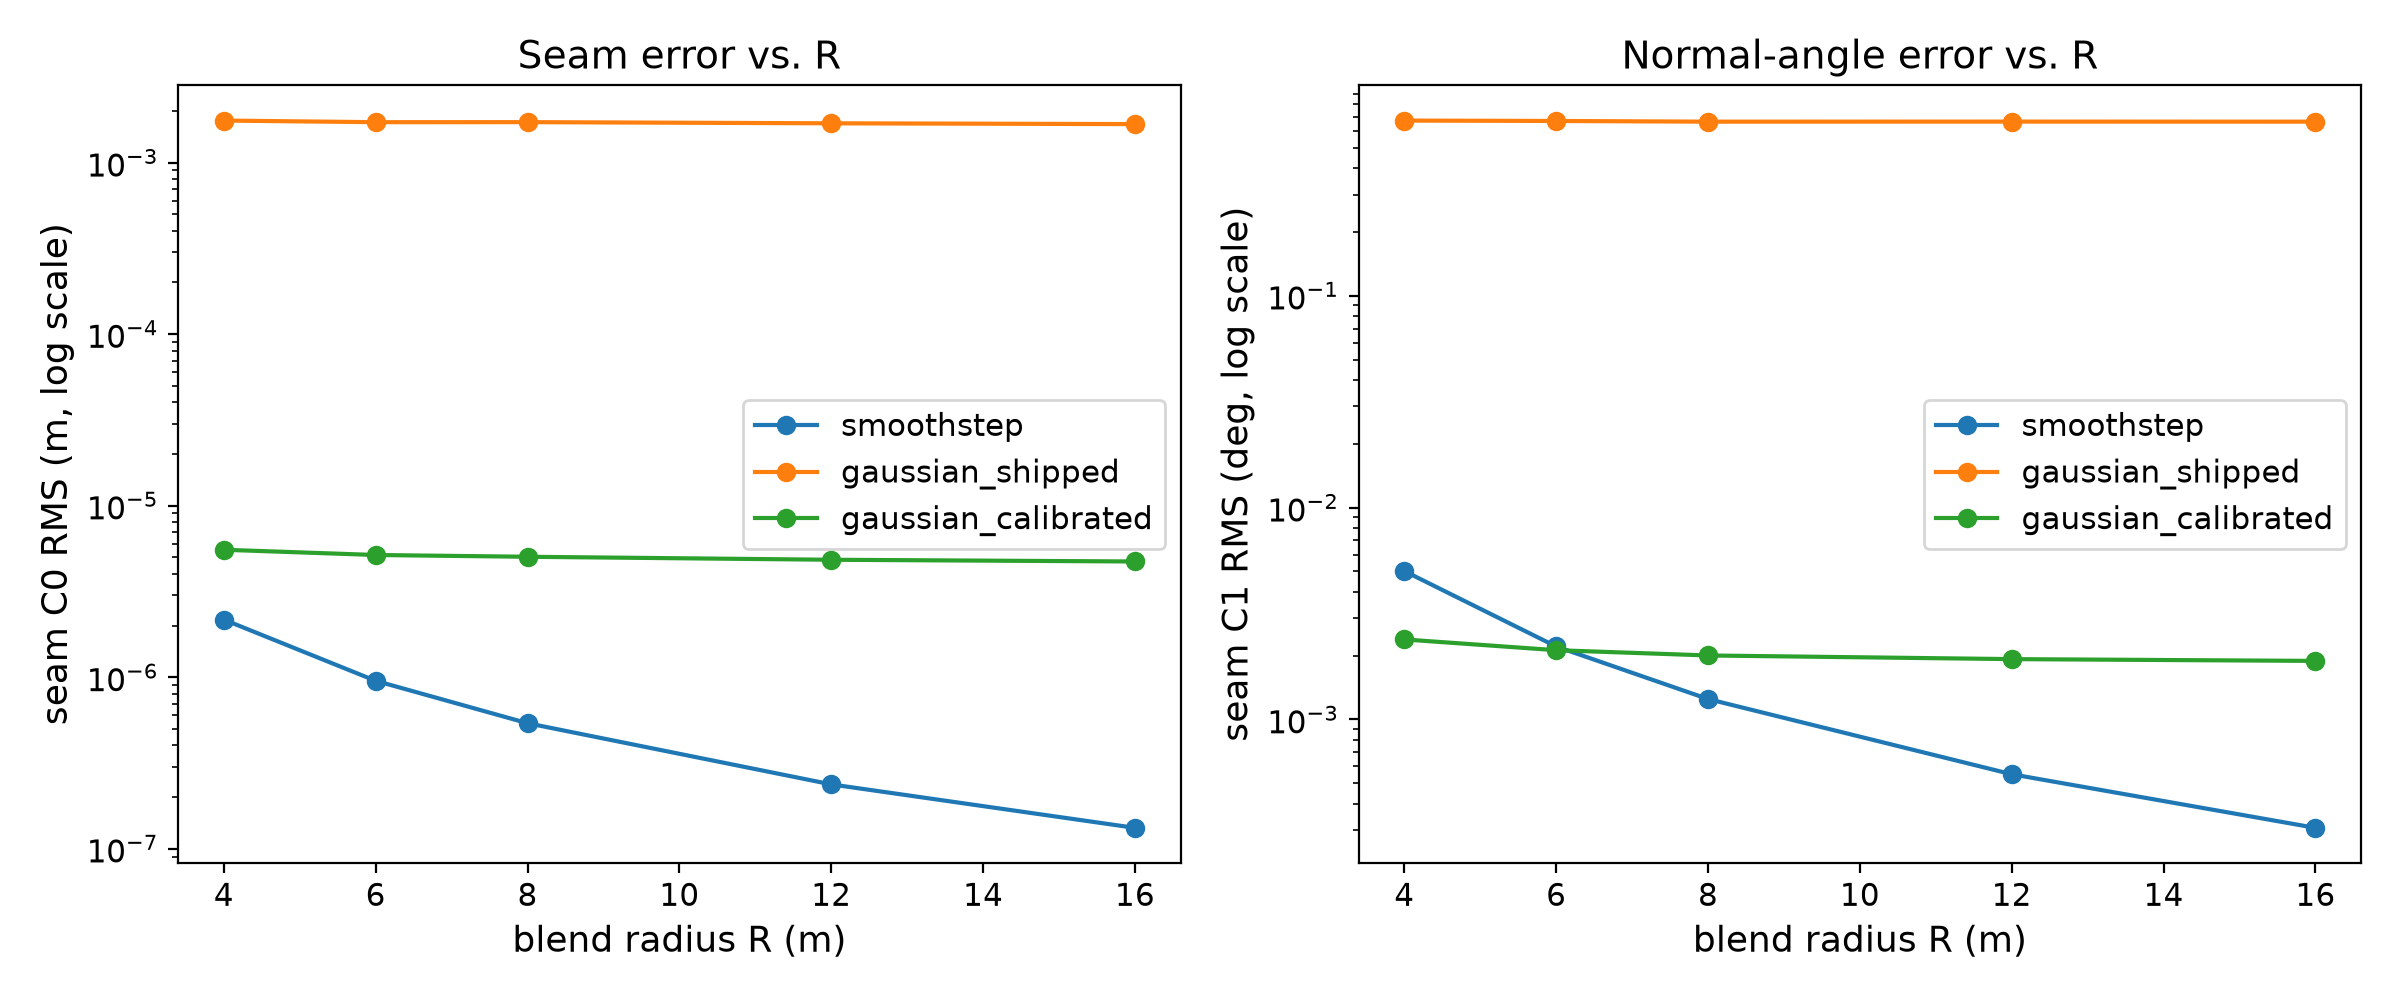
\includegraphics[width=0.92\linewidth]{radius_sweep.png}
  \caption{Transition-radius ($R$) sweep: scale invariance}
  \label{fig:rsweep}
\end{figure}

In the grid-resolution sweep (grid spacing roughly 0.31-1.27 m; Figure~\ref{fig:ressweep}), the empirical convergence order (slope of the log-log linear regression) of the \texttt{smoothstep} and \texttt{hybrid} methods was measured at roughly 0.90, i.e. the error decreases as expected as resolution increases. For the calibrated Gaussian, a negative slope (roughly -0.36) was observed; however, this is not a physical "worsens as resolution increases" finding~--- the calibrated Gaussian's error is already on the order of 1e-6 to 1e-7 m, close to a fixed truncation-residual noise floor set by the calibration constant, and this floor constitutes a measurement limit independent of grid resolution; this point is stated explicitly here to avoid a misleading physical interpretation.

\begin{figure}[htb]
  \centering
  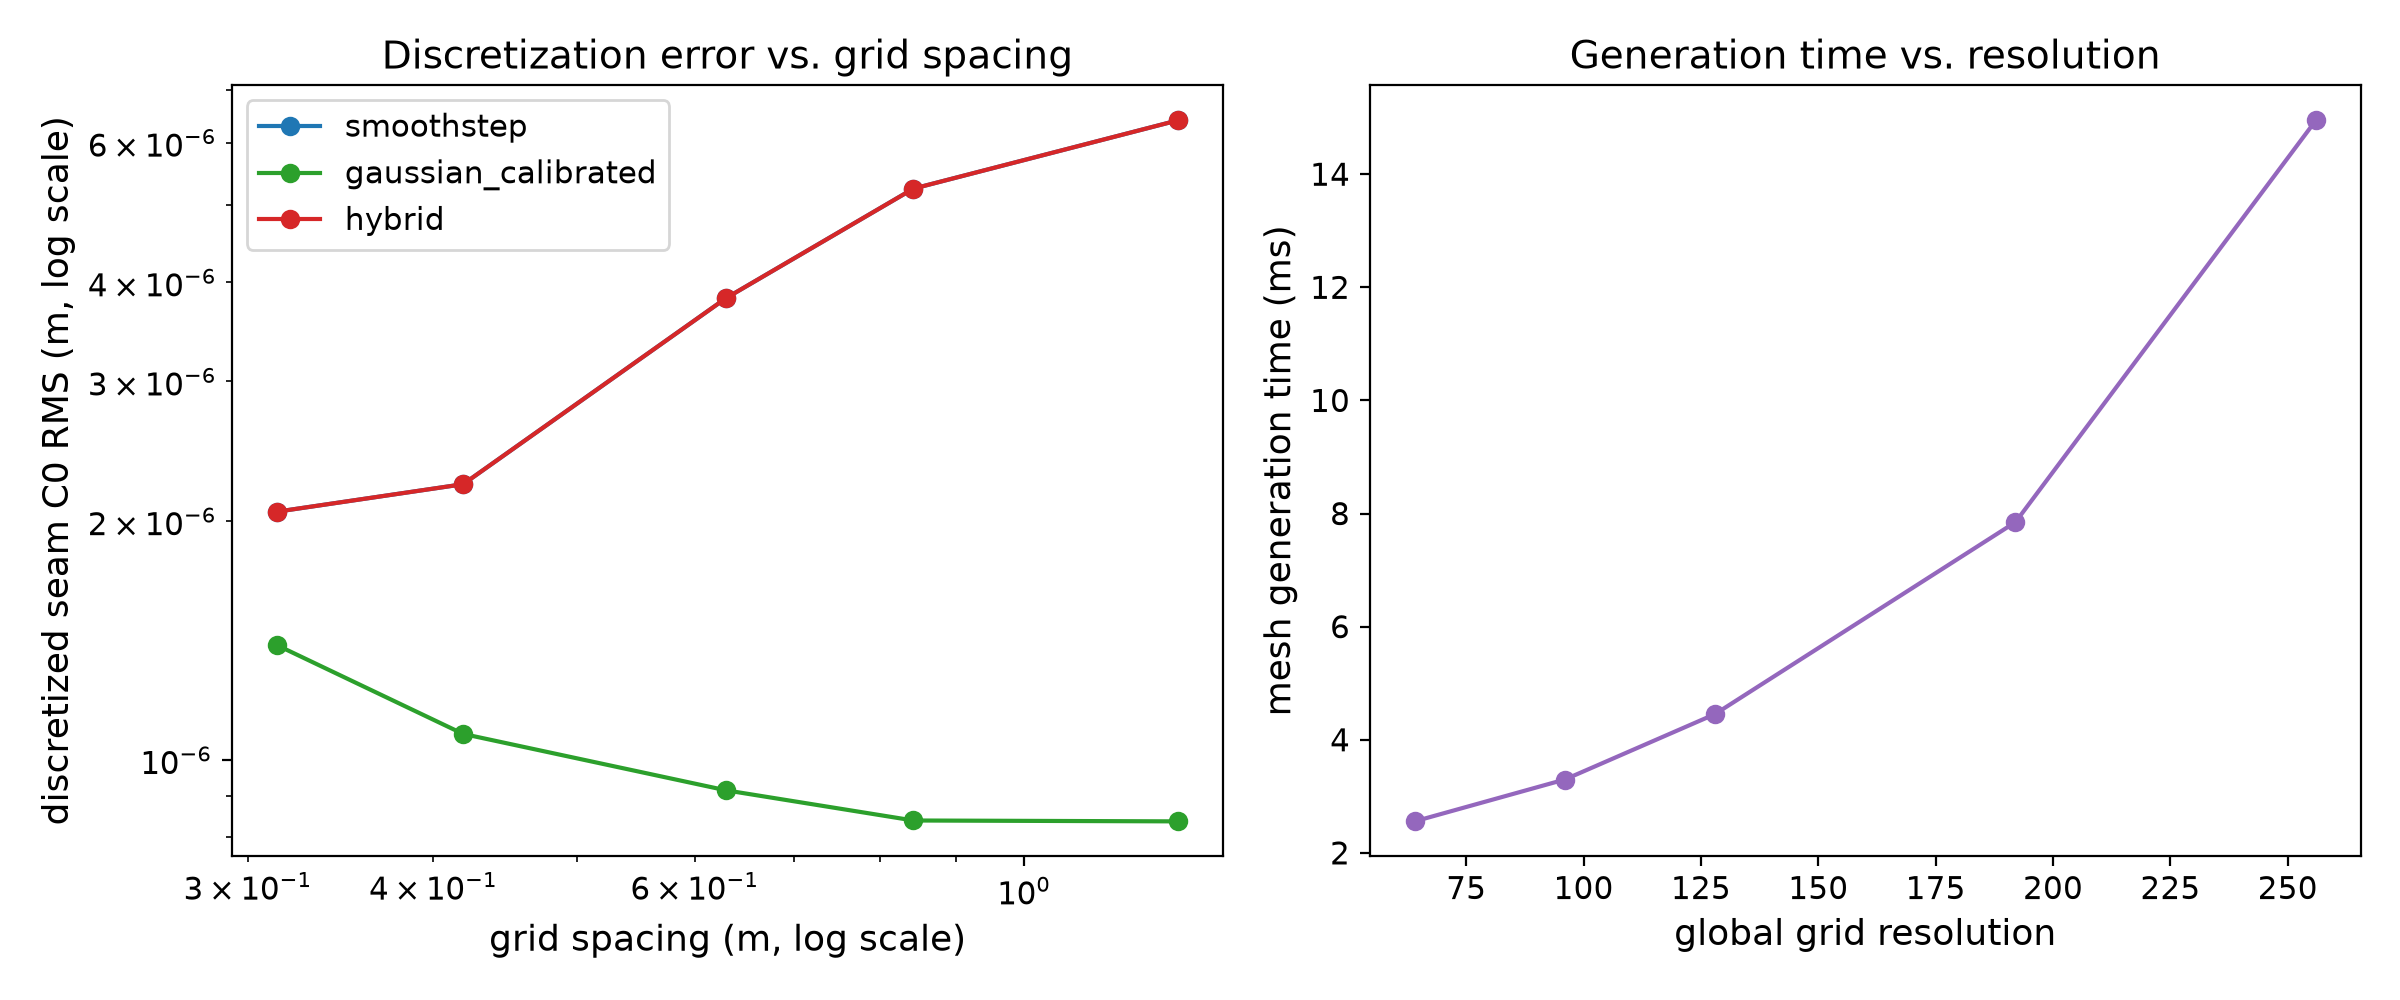
\includegraphics[width=0.92\linewidth]{resolution_sweep.png}
  \caption{Grid-resolution sweep: empirical convergence order}
  \label{fig:ressweep}
\end{figure}

The common conclusion of the four analyses is that the continuity advantage of the proposed \texttt{hybrid} method is robust over a reasonable parameter range (rc = 1.0-4.0 m, w = 0.3-1.0 m), i.e. it is not overly sensitive to a particular fine-tuning. The only exception is that at very narrow switch widths (w <= 0.1 m) the internal continuity degrades noticeably; this once again confirms that the default used in the production configuration (w = 0.3 m) contains a deliberate safety margin.


\subsection{Isaac Sim Training Results}\label{sec:rlresults}
All nine training runs (3 methods x 3 seeds) completed without error, each reaching 5,734,400 environment steps (Table~\ref{tab:rlsummary}). The wall-clock time, as a method average, is 2377 +- 98 seconds for \texttt{smoothstep}, 2850 +- 898 seconds for the calibrated Gaussian, and 2674 +- 599 seconds for the \texttt{hybrid}. These averages show that the large difference observed in the first (seed=42) runs (Gaussian and \texttt{hybrid} 56\% and 35\% slower respectively) shrank substantially with multiple seeds: the three seed=7 and seed=123 runs all took similar times (2318-2345 seconds), while only the Gaussian and \texttt{hybrid} runs at seed=42 are markedly slower. The magnitude of the standard deviations (898 and 599 seconds, 20-30\% of the mean) is the source of this single-run deviation; the first measurement's "35-56\% slower" finding may therefore stem not from the blending formula itself but from a system-level variability specific to that particular run (background load, thermal state, or terrain-pool timing); averaged over the three seeds, the Gaussian and \texttt{hybrid} still appear slower than \texttt{smoothstep} (+20\% and +12.5\%), but this difference is no longer as sharp as in the first measurement.

\begin{table}[htb]
\centering
\caption{Final ten-percent window summary in the real Isaac Sim training, three seeds per method. All rate columns are mean $\pm$ standard deviation over the three seeds; \emph{Curric.} is the curriculum difficulty reached.}
\label{tab:rlsummary}
\footnotesize
\setlength{\tabcolsep}{3pt}
\begin{tabular}{@{}lrrrrrr@{}}
\toprule
Method & n & Wall time (s) & Success & Timeout & Harsh & Curric. \\
\midrule
\texttt{smoothstep} & 3 & 2377 +- 98 & 0.278 +- 0.055 & 0.499 +- 0.059 & 0.220 +- 0.022 & 0.276 +- 0.025 \\
\texttt{gaussian} (calibrated) & 3 & 2850 +- 898 & 0.325 +- 0.051 & 0.454 +- 0.074 & 0.218 +- 0.038 & 0.250 +- 0.000 \\
\texttt{hybrid} & 3 & 2674 +- 599 & 0.268 +- 0.025 & 0.515 +- 0.019 & 0.214 +- 0.007 & 0.260 +- 0.017 \\
\bottomrule
\end{tabular}
\end{table}


The final success rate measured in the final ten-percent window was, as a method average, 27.8\% +- 5.5\% for \texttt{smoothstep}, 32.5\% +- 5.1\% for the calibrated Gaussian, and 26.8\% +- 2.5\% for the \texttt{hybrid} (Table~\ref{tab:rlsummary}). The Gaussian's mean is still the highest, but the standard deviations of the three methods overlap with each other. Table~\ref{tab:rlstats} summarizes the pairwise statistical tests of these differences: no pairwise comparison is statistically significant; on success rate, \texttt{smoothstep}-Gaussian p=0.20, \texttt{smoothstep}-\texttt{hybrid} p=1.00, Gaussian-\texttt{hybrid} p=0.40; on timeout rate, p=0.70, p=1.00, p=0.40 respectively; on harsh-landing rate, all three p>=0.70. All of the bootstrap 95\% confidence intervals include zero (e.g. [-0.000, 0.104] for the Gaussian-\texttt{hybrid} success-rate difference~--- borderline but containing zero).

\begin{table}[htb]
\centering
\caption{Pairwise comparisons over the final ten-percent window (Mann--Whitney U, descriptive; see the caveat in Section~\ref{sec:rlprotocol}). All comparisons are 3 seeds versus 3 seeds.}
\label{tab:rlstats}
\footnotesize
\setlength{\tabcolsep}{4pt}
\begin{tabular}{@{}llrrlr@{}}
\toprule
Metric & Comparison & n & Mean diff & 95\textbackslash{}\% CI & p \\
\midrule
Success rate & \texttt{smoothstep} vs \texttt{gaussian} & 3 vs 3 & -0.047 & [-0.112, 0.018] & 2.00e-01 \\
Success rate & \texttt{smoothstep} vs \texttt{hybrid} & 3 vs 3 & 0.010 & [-0.040, 0.068] & 1.00e+00 \\
Success rate & \texttt{gaussian} vs \texttt{hybrid} & 3 vs 3 & 0.057 & [-0.000, 0.104] & 4.00e-01 \\
Timeout rate & \texttt{smoothstep} vs \texttt{gaussian} & 3 vs 3 & 0.045 & [-0.044, 0.133] & 7.00e-01 \\
Timeout rate & \texttt{smoothstep} vs \texttt{hybrid} & 3 vs 3 & -0.017 & [-0.073, 0.039] & 1.00e+00 \\
Timeout rate & \texttt{gaussian} vs \texttt{hybrid} & 3 vs 3 & -0.061 & [-0.132, 0.008] & 4.00e-01 \\
Harsh-landing rate & \texttt{smoothstep} vs \texttt{gaussian} & 3 vs 3 & 0.002 & [-0.041, 0.040] & 1.00e+00 \\
Harsh-landing rate & \texttt{smoothstep} vs \texttt{hybrid} & 3 vs 3 & 0.006 & [-0.012, 0.031] & 1.00e+00 \\
Harsh-landing rate & \texttt{gaussian} vs \texttt{hybrid} & 3 vs 3 & 0.004 & [-0.027, 0.047] & 7.00e-01 \\
\bottomrule
\end{tabular}
\end{table}


Figure~\ref{fig:trainmetrics} shows all nine runs of the three methods on the same plot for the three main outcome metrics (success, timeout, harsh-landing rate); the nine curves being largely intertwined throughout training confirms that the difference among methods cannot be distinguished visually from the variance across seeds. Figure~\ref{fig:traindiag} shows, for the same nine runs, complementary training diagnostics such as curriculum difficulty, entropy coefficient, and xy-progress reward; the entropy coefficient following an almost identical convergence curve for all three methods indicates that SAC's exploration-exploitation balance operates independently of the choice of blending method. Figure~\ref{fig:boxplot} presents the final ten-percent window values as per-method scatter points and a mean +/- standard deviation bar; the wide overlap of the three methods' error bars is also clearly visible here.

\begin{figure}[htb]
  \centering
  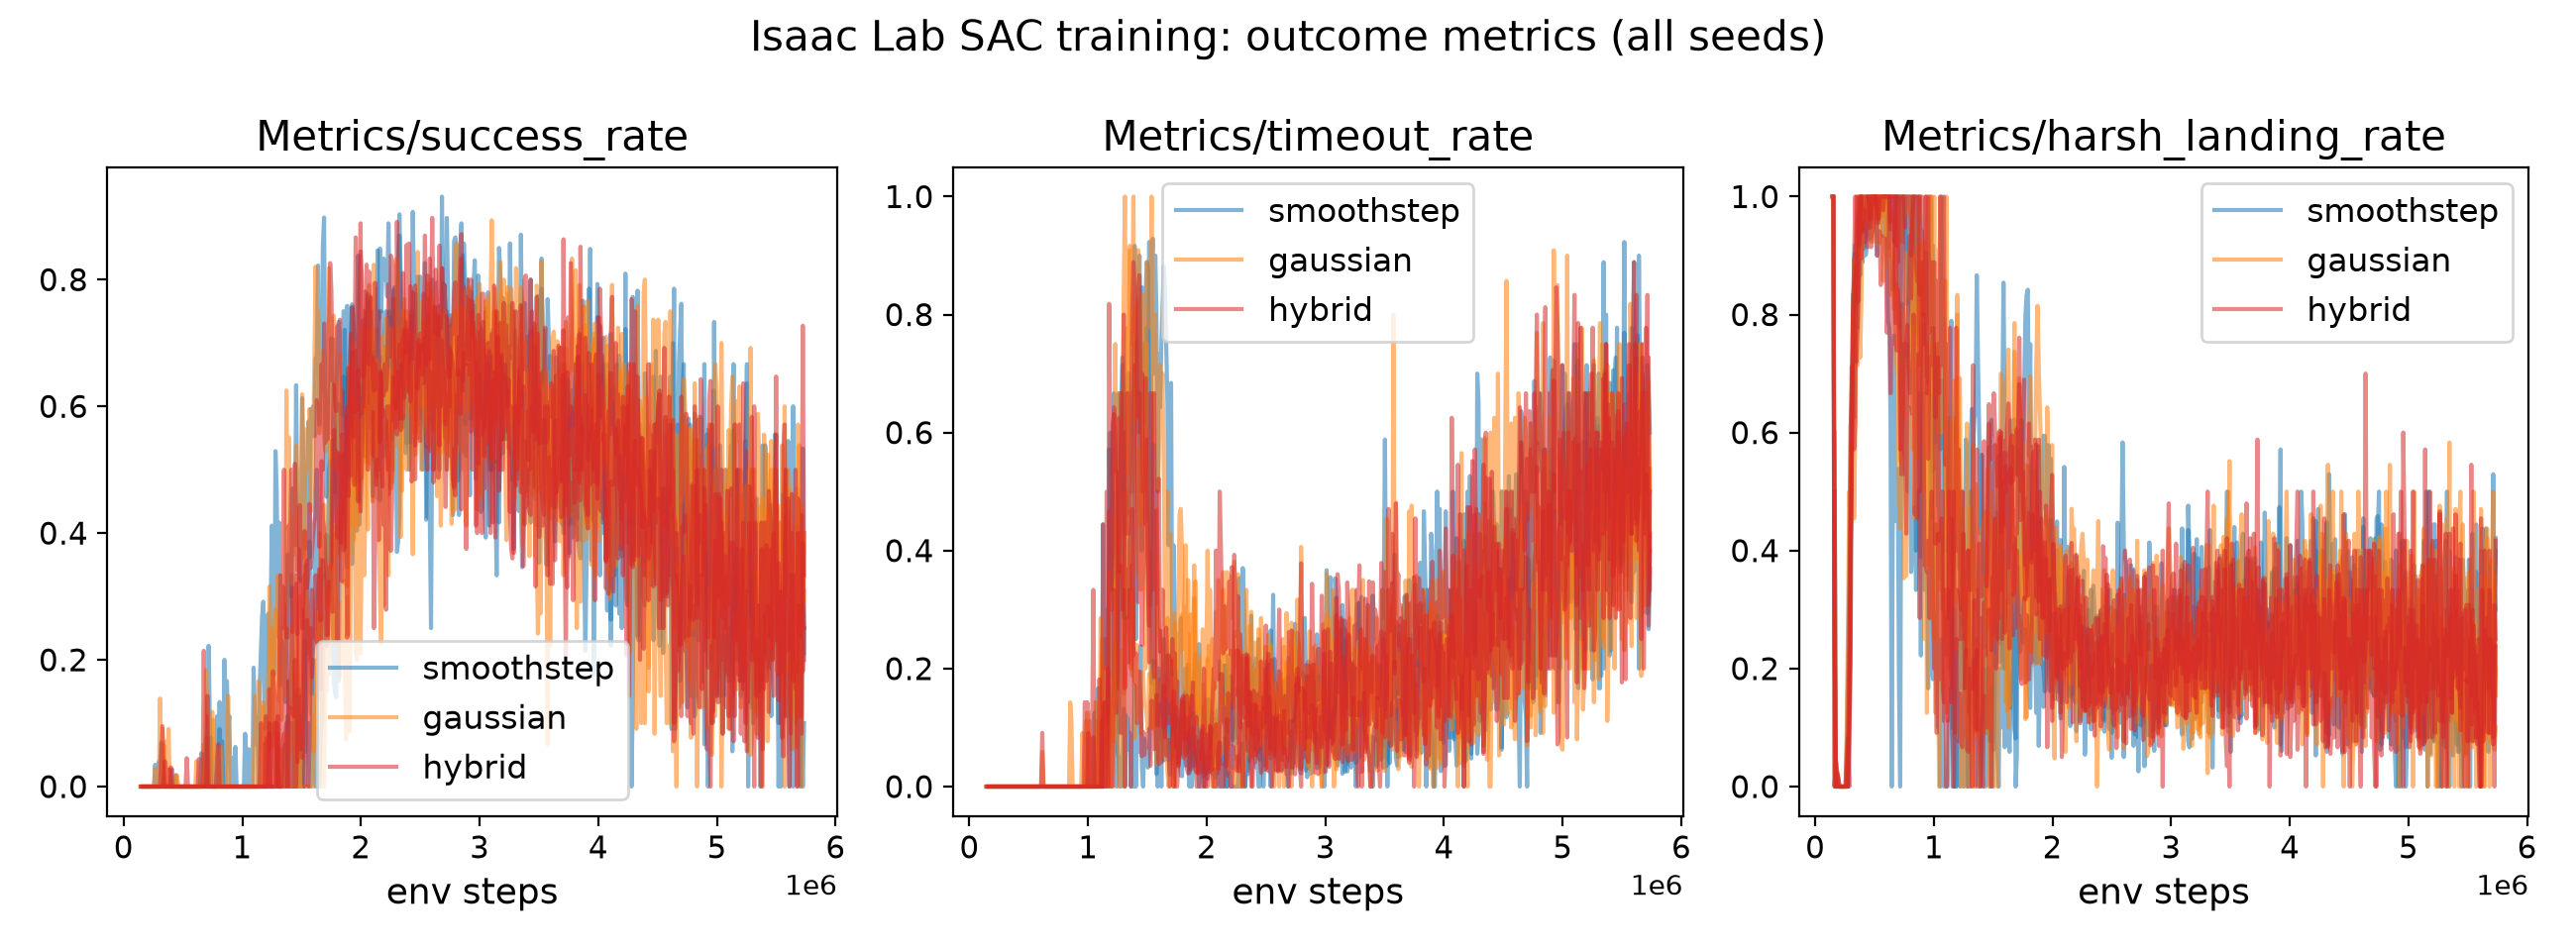
\includegraphics[width=0.96\linewidth]{training_comparison_metrics.png}
  \caption{Outcome metrics tracked over training for the three methods
  (success/timeout/harsh-landing rate)}
  \label{fig:trainmetrics}
\end{figure}

\begin{figure}[htb]
  \centering
  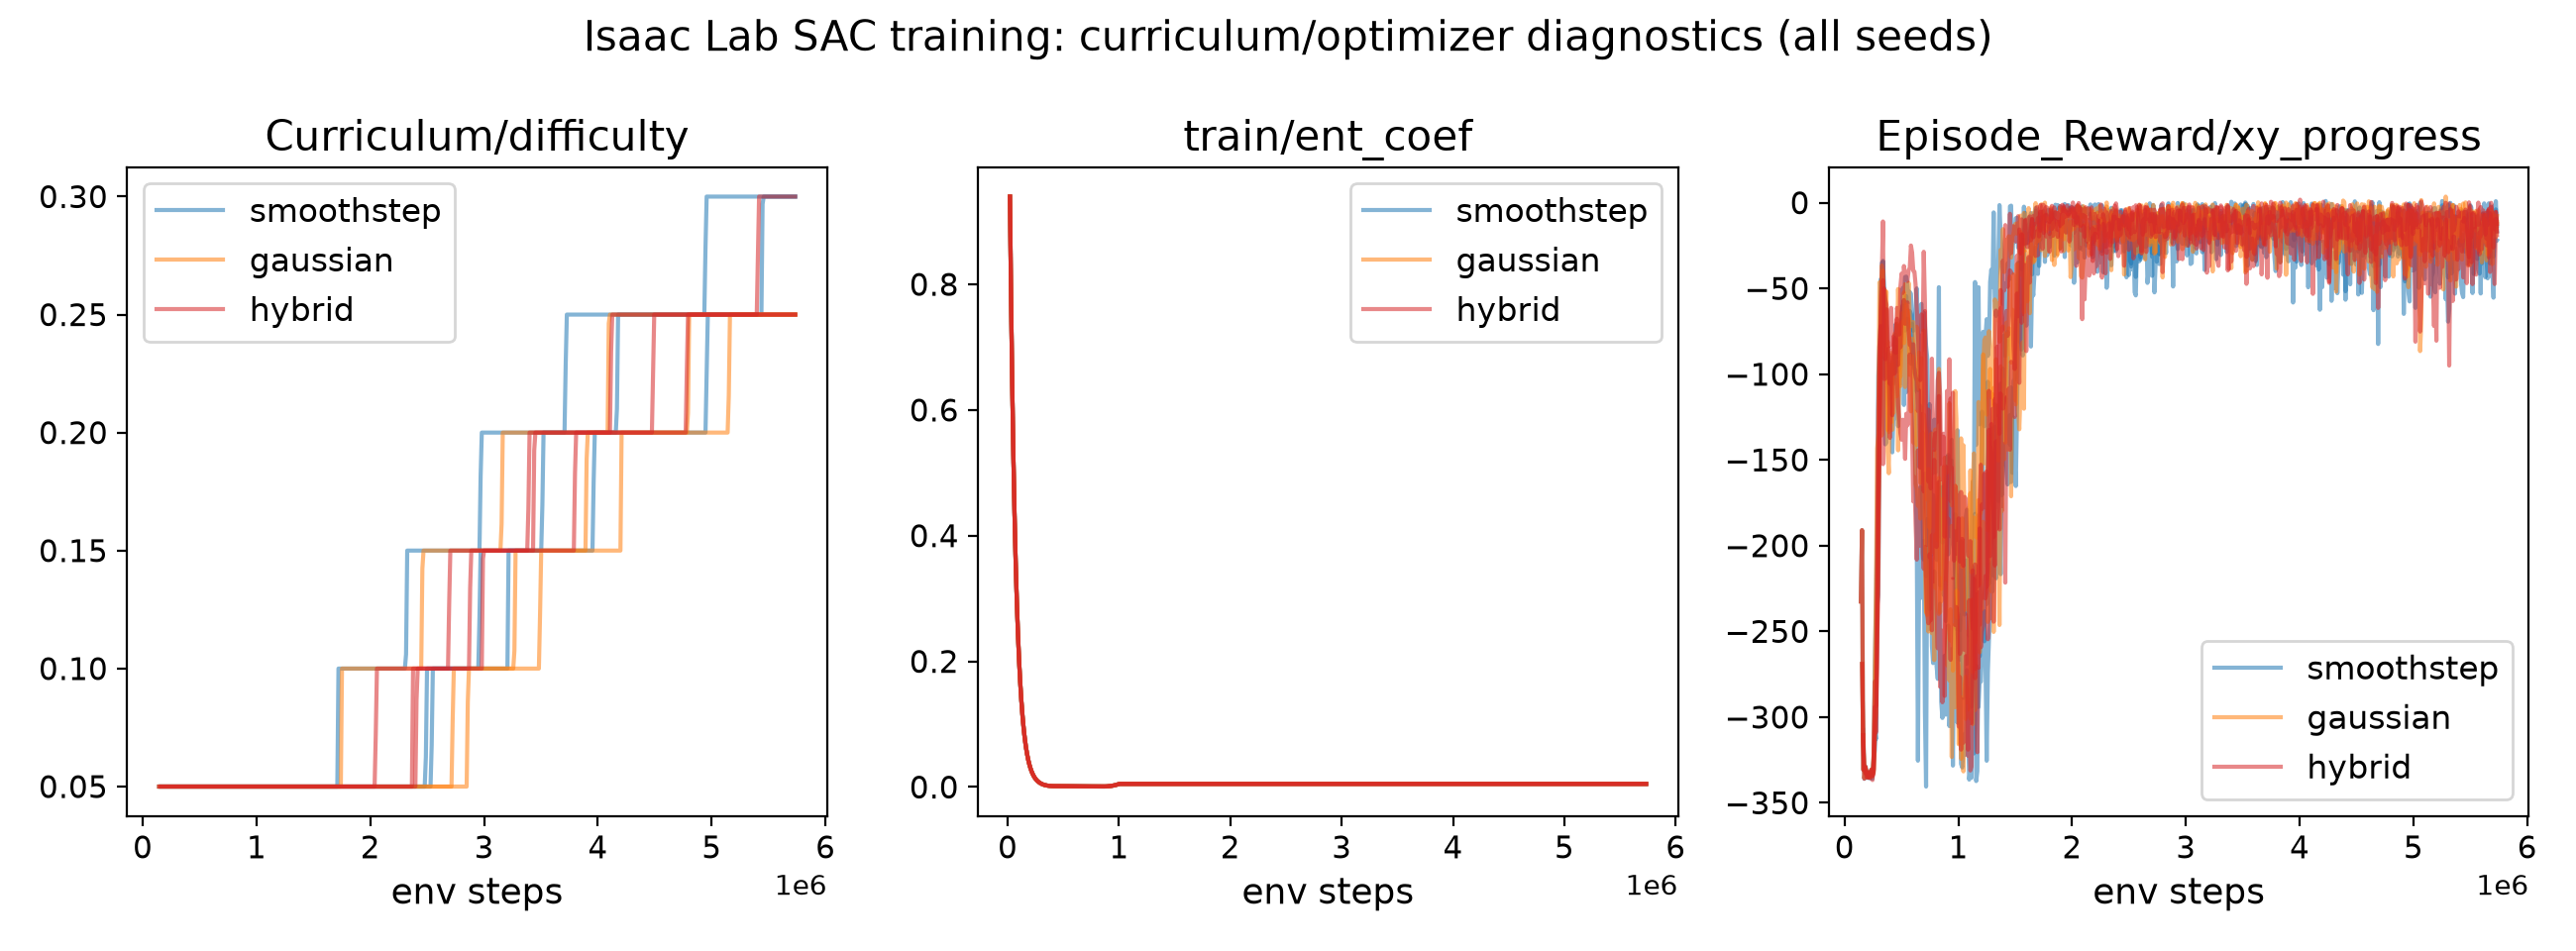
\includegraphics[width=0.96\linewidth]{training_comparison_diagnostics.png}
  \caption{Complementary diagnostics tracked over training for the three
  methods (curriculum difficulty, entropy coefficient, xy-progress reward)}
  \label{fig:traindiag}
\end{figure}

\begin{figure}[htb]
  \centering
  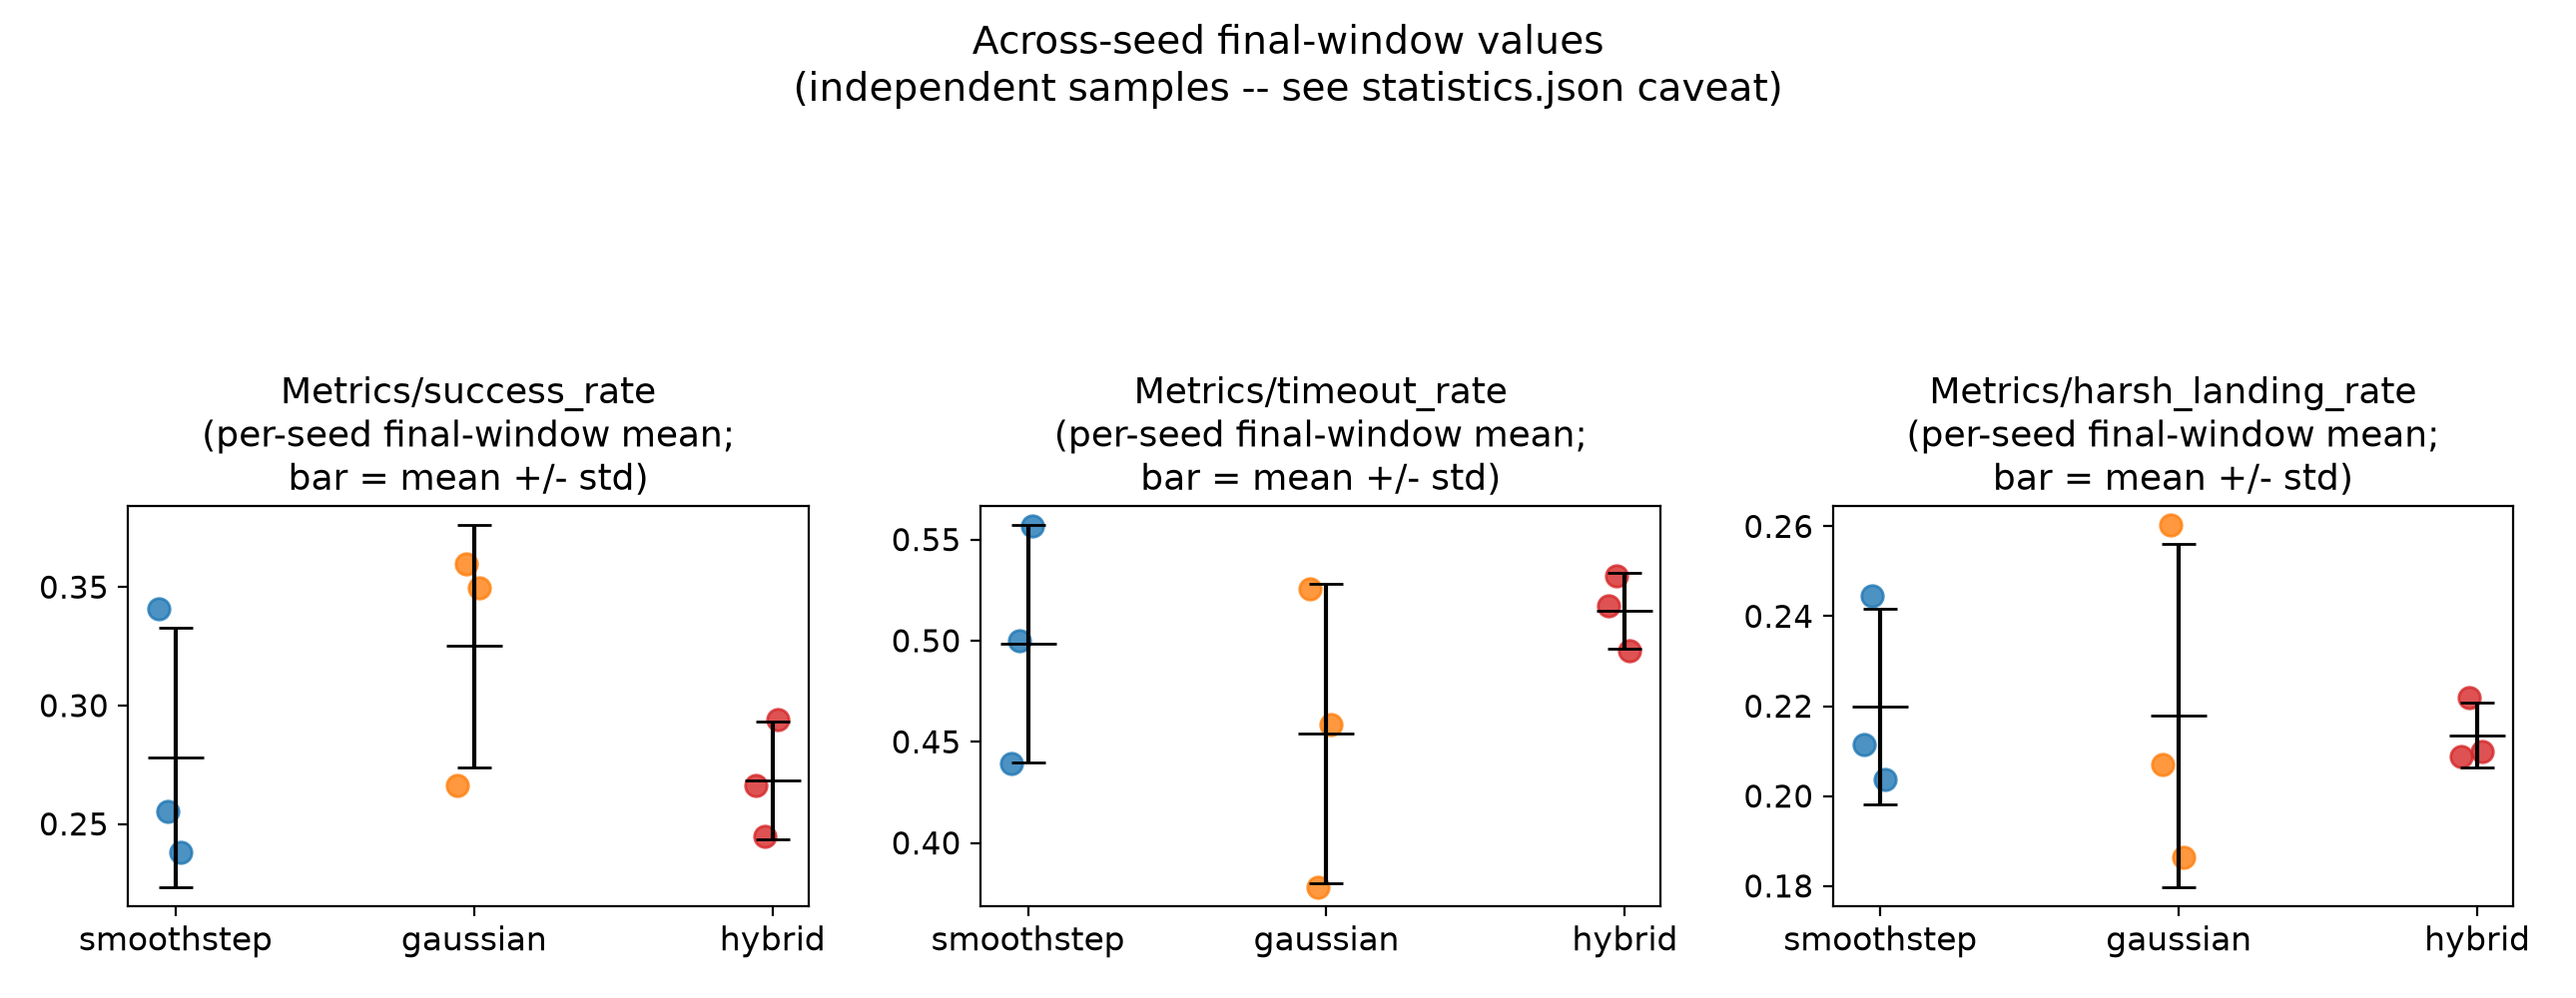
\includegraphics[width=0.86\linewidth]{final_window_boxplot.png}
  \caption{Final ten-percent window distributions (box plot)}
  \label{fig:boxplot}
\end{figure}

This result does not confirm the finding, observed in the first (single-seed) measurement and discussed in detail in Section~\ref{sec:discussion}, that "the Gaussian and \texttt{hybrid} are significantly more successful than \texttt{smoothstep}." Going from n=1 to n=3, the effect size shrank (the Gaussian-\texttt{smoothstep} difference dropped from 11\% to 4.7\%) and the direction partly changed (the \texttt{hybrid}-\texttt{smoothstep} difference changed sign: in the first measurement the \texttt{hybrid} was higher than \texttt{smoothstep}, while in the three-seed average the \texttt{hybrid} is almost equal to \texttt{smoothstep}, even slightly lower). This pattern shows that the first finding is~--- at least largely~--- consistent with random run-to-run variance; this point is discussed in detail in Section~\ref{sec:discussion}. It is also the behaviour the reinforcement learning methodology literature predicts: \citet{colas2018} show that the seed counts typically reported are far below the statistical power needed to resolve differences of this size, and \citet{agarwal2021} demonstrate that point estimates computed from a handful of runs routinely reverse once uncertainty is reported properly.

The sample-efficiency measures show a similar picture: the AUC (mean success rate over training) varies over a wide range across the three seeds per method (\texttt{smoothstep} 0.381-0.395, Gaussian 0.366-0.402, \texttt{hybrid} 0.339-0.399), and the difference among methods is markedly smaller than the difference across seeds~--- again indicating that seed variance is the dominant source.

Curriculum difficulty is on average close among the three methods (\texttt{smoothstep} 0.276 +- 0.025, Gaussian 0.250 +- 0.000, \texttt{hybrid} 0.260 +- 0.017); it is notable that the Gaussian stays exactly at 0.25 on all three seeds (zero standard deviation), showing that the rolling-window success threshold stopped at the same step in all three of those runs~--- this is consistent with the observation, put forward in the first measurement, that "the Gaussian lags behind in the curriculum despite its high mean success," although the cause was not directly tested.


\section{Discussion}\label{sec:discussion}
The findings give, first of all, a clear answer to RQ1: the seam left by the as-shipped Gaussian blend when truncated at a finite radius is not a cosmetic or negligible defect but a measurable and statistically extremely significant structural defect, roughly three orders of magnitude worse than \texttt{smoothstep} (about 3200x on C0, 530x on C1). The source of this defect is not a coding error but a property of radial basis functions known for more than fifty years: the Gaussian-type radial functions defined by \citet{hardy1971} are infinite-support and never reach exactly zero at any finite radius; \citet{wendland1995} proposed compact-support, minimal-degree positive-definite radial functions precisely as the solution to this problem. The contribution of this study is to demonstrate this fifty-year-old mathematical knowledge quantitatively in a concrete engineering setting (a physically queryable lunar-surface height field) and to test whether it is reflected in an RL training run. This analytic finding, unlike the RL results discussed below, is validated with 30 seeds and is not subject to single-run uncertainty; it is therefore the study's most robust, least contentious finding.

In answer to RQ2, the proposed \texttt{hybrid} method preserves the Gaussian's soft "bell" profile in the contact region and \texttt{smoothstep}'s compact support beyond it, while creating no new seam at its own internal transition (switch); this is an expected result consistent with the partition-of-unity framework described by \citet{ohtake2003}: the convex combination of two C1-smooth functions with a C1-smooth weight is again C1-smooth. The price of this advantage is a microsecond cost roughly 4.3 times that of \texttt{smoothstep} in computing the pure fade formula (because both branches are computed). This formula-level cost is reflected only partially and inconsistently in the real training wall-clock time: in the first (seed=42) measurement the Gaussian and \texttt{hybrid} were 56\% and 35\% slower respectively, but averaged over the three seeds this difference drops to 20\% and 12.5\%, and the standard deviation (20-30\% of the mean) shows how much a single run can deviate (Section~\ref{sec:rlresults}). This suggests that the real wall-clock difference stems largely from run-to-run system variability (background load, thermal state, terrain-pool timing), with the pure formula cost contributing only a small and consistent amount; this is a separate observation, one that should not be over-interpreted but that shows single-run measurements can also be misleading in cost comparisons.

The answer to RQ3 changed substantially after multiple seeds, and that change is itself one of the study's most instructive findings. In the first (single-seed, seed=42) measurement, the Gaussian and \texttt{hybrid} appeared to reach a final success rate roughly 8-12 percentage points higher than \texttt{smoothstep}, and in the first draft this was attributed to a mechanism such as a "difference in the transition-band weight profile." In the measurement extended with two additional independent seeds (seed=7, seed=123) (Section~\ref{sec:rlresults}), the difference among methods shrank (the Gaussian-\texttt{smoothstep} difference from 11\% to 4.7\%), the \texttt{hybrid}-\texttt{smoothstep} difference changed sign, and no pairwise comparison came out statistically significant on any of the three metrics (success rate, timeout rate, harsh-landing rate) (all p>=0.20). Recalling that the analytic boundary continuity of the Gaussian variant used in the real training (calibrated, k=ln(1000)) is already almost equal to \texttt{smoothstep} (Table~\ref{tab:continuity}), this result actually shows an expected consistency: if there is no measurable difference in boundary continuity, it is no surprise that there is no strong difference in RL training performance either. The apparent difference in the first measurement was most likely ordinary run-to-run variance stemming from the inherent nondeterminism of the GPU-parallel PhysX simulation and of the terrain pool's background CPU generation process~--- exactly the pseudoreplication pitfall \citet{henderson2018} warn about. Because this study refuted its own initial finding in this way, it provides an in-house case study of how misleading single-run RL comparisons can be: going from n=1 to n=3 was enough to turn a seemingly "significant" finding into a statistically indistinguishable one. That said, n=3 is still low-powered, and the current data cannot rule out the existence of a small real effect either (in particular, the Gaussian consistently having the highest mean); reaching a firm conclusion requires more seeds (Section~\ref{sec:conclusion}).

The scope of this study was deliberately kept narrow so that the effect of the blending function could be isolated as a single variable; the three methods were compared only with each other, holding the rest of the production environment (physics engine, reward function, agent architecture, curriculum) fixed. Porting another terrain-blending method from the literature~--- e.g. one implemented in another simulator~--- directly into this environment as an external benchmark was deliberately not chosen; such a benchmark would make it impossible to separate the effect of the blending function from the countless other differences in that simulator's physics engine, observation/reward design, and agent architecture. The cost of this is that the extent to which the findings generalize beyond this specific environment (Isaac Lab/PhysX, SAC, this task definition)~--- the external validity~--- is not tested in this study; this point is addressed as a concrete future-work direction in Section~\ref{sec:conclusion}.

The most important limitation of this study is that it still has low statistical power with n=3: with the current data, the smallest p value the Mann-Whitney test can produce is already limited (around a minimum of p=0.10 in a 3-versus-3 comparison), so the "no significant difference" finding does not prove that the methods are genuinely equivalent~--- it only shows that the large apparent difference in the first measurement could not be reliably confirmed. \citet{colas2019} make the remedy explicit: a comparison of this kind should either report interval estimates rather than point estimates, or state in advance the effect size it is powered to detect, and the present design does neither. A second limitation is that the training scale (5.73 million steps, roughly 350 iterations) is below the full-scale configuration (1200 iterations) because of the compute budget; no run may have reached full convergence, which means the observed plateaus may reflect an interim performance difference rather than a final/asymptotic one. A third limitation is that the analytic/CPU study isolates only the fade formula itself and does not fully separate the source of the real training wall-clock difference (terrain generation, physics stepping, system variability)~--- although the three-seed data shows this difference shrinking, it does not pin down its source with certainty.


\section{Conclusion}\label{sec:conclusion}
This study systematically examined the shape of the blending function used at the boundary where a coarse global terrain and a fine-detail local patch meet, in an Isaac Lab-based lunar landing environment, both at the analytic/CPU level and in a real Isaac Sim SAC training run. Analytic measurements over many seeds showed, with statistical significance, that the previously used as-shipped Gaussian blend produces boundary continuity worse than \texttt{smoothstep} by several orders of magnitude when truncated at a finite radius, and that this defect is a scale-invariant, structural property. The proposed \texttt{hybrid} method and a calibrated Gaussian variant both removed this defect to near machine precision; this is the study's most robust and least contentious finding.

The real training comparison began with a single seed per method and, in that first measurement, showed the Gaussian and \texttt{hybrid} reaching a markedly higher success rate than \texttt{smoothstep}. Extending the study with additional independent seeds found no statistically significant difference among the methods on any metric, which turns the first measurement into a concrete, self-sourced example of how misleading single-run RL comparisons can be. Taken together with the analytic results, the choice of blending function has a measurable and robust effect on boundary continuity, but at this scale that effect is not distinguishable in final training performance. All three methods are integrated into the production code as a backward-compatible, selectable configuration, so the choice can rest on other criteria such as boundary continuity, which favours the Gaussian and \texttt{hybrid}, or computational cost, which favours \texttt{smoothstep}.

Three concrete directions are proposed for future work. First, the real training comparison should be extended with substantially more independent seeds, to determine whether the small mean differences observed, in particular the Gaussian consistently having the highest mean, are a real effect or residual noise. Second, the training scale should be raised to the full configuration, to confirm whether the observed plateaus reflect a final rather than an interim performance difference. Third, the external validity of the findings should be tested by repeating the same three blending methods on another physics engine, another reward and observation design, or another contact-rich task such as quadruped locomotion or humanoid standing.

